% arara: pdflatex: { synctex: yes }
% arara: makeindex: { style: ctuthesis }
%% arara: bibtex
%\listfiles
%\PassOptionsToPackage{cp1250}{inputenc}
% The class takes all the key=value arguments that \ctusetup does,
% and couple more: draft and oneside
\documentclass[twoside]{ctuthesis}
\makeatletter
\edef\mytoday{\expandafter\@gobbletwo\the\year\ifnum\month<10 0\fi\the\month\ifnum\day<10 0\fi\the\day}
\makeatother
% LaTeX logo with better kerning in sf bf font
\makeatletter
\newcommand\LaTeX@lmss@bx{L\kern -.33em{\sbox \z@ T\vbox to\ht \z@ {\hbox {\check@mathfonts \fontsize \sf@size \z@ \math@fontsfalse \selectfont A}\vss }}\kern -.15em\TeX}
\DeclareRobustCommand\myLaTeX{%
        \ifcsname LaTeX@\f@family @\f@series\endcsname
                \csname LaTeX@\f@family @\f@series\endcsname
        \else
                \LaTeX
        \fi
}
\usepackage{datetime}
\ctusetup{
%       preprint = {\ctuverlog \\ ctuman \mytoday},
        mainlanguage = english,
        titlelanguage = english,
        otherlanguages = {english, czech},
        title-czech = {Hluboké neuronové sítě ve vestavěných systémech},
        title-english = {Deep Neural Networks in Embedded Systems},
        doctype-czech = {Diplomová práce},
        doctype-english = {Master's Thesis},
        xfaculty = F3,
        department-czech = {Katedra kybernetiky},
        department-english = {Department of Cybernetics},
        author = {Bc. Mykhaylo Zelenskyy},
        supervisor = {Ing. Lukáš Hrubý},
%       supervisor-address = {Ústav X, \\ Uliční 5, \\ Praha 99},
        keywords-czech = {},
        keywords-english = {},
        day = \the\day,
        month = \the\month,
        year = \the\year,
%       list-of-figures = false,
%       list-of-tables = false,
%       monochrome = true,
%       savetoner = true,
        pkg-listings = true,
        ctulstbg = none,
%       layout-short = true,
%       pkg-hyperref = false,
}
\ctuprocess
% Theorem declarations, this is the reasonable default, anybody can do what they wish.
% If you prefer theorems in italics rather than slanted, use \theoremstyle{plainit}
\theoremstyle{plain}
\newtheorem{theorem}{Theorem}[chapter]
\newtheorem{corollary}[theorem]{Corollary}
\newtheorem{lemma}[theorem]{Lemma}
\newtheorem{proposition}[theorem]{Proposition}
\theoremstyle{definition}
\newtheorem{definition}[theorem]{Definition}
\newtheorem{example}[theorem]{Example}
\newtheorem{conjecture}[theorem]{Conjecture}
\theoremstyle{note}
\newtheorem*{remark*}{Remark}
\newtheorem{remark}[theorem]{Remark}
\DeclareMathOperator{\atantwo}{atan2}
% Marginpars used as navigation aids.
%\PassOptionsToPackage{table,xcdraw}{xcolor}
\usepackage{colortbl}
\usepackage{tikz}
\usepackage{mparhack}
\usepackage{epstopdf}
\usepackage{subfig}
\usepackage{siunitx}
\usepackage{url}
\usepackage{multirow}
\usepackage[justification=centering]{caption}
\usepackage{amsmath}
\usepackage[framemethod=tikz]{mdframed}
\usepackage{url}
\usepackage{hyperref}
%\usepackage{degrade}
\usepackage{graphicx}
\usepackage{hhline}
\usepackage[edges]{forest}
\usepackage{textcomp}
\usepackage{tabularx}
\usepackage{perpage} %the perpage package
\MakePerPage{footnote} %the perpage package command
\newcommand{\norm}[1]{\left\lVert#1\right\rVert}
\definecolor{folderbg}{RGB}{124,166,198}
\definecolor{folderborder}{RGB}{110,144,169}
\definecolor{foldercolor}{RGB}{124,166,198}
\def\Size{4pt}
\tikzset{pics/folder/.style={code={%
                        \node[inner sep=0pt, minimum size=#1](-foldericon){};
                        \node[folder style, inner sep=0pt, minimum width=0.3*#1, minimum height=0.6*#1, above right, xshift=0.05*#1] at (-foldericon.west){};
                        \node[folder style, inner sep=0pt, minimum size=#1] at (-foldericon.center){};}
        },
        pics/folder/.default={20pt},
        folder style/.style={draw=foldercolor!80!black,top color=foldercolor!40,bottom color=foldercolor}
}
\forestset{is file/.style={edge path'/.expanded={%
                        ([xshift=\forestregister{folder indent}]!u.parent anchor) |- (.child anchor)},
                inner sep=1pt},
        this folder size/.style={edge path'/.expanded={%
                        ([xshift=\forestregister{folder indent}]!u.parent anchor) |- (.child anchor) pic[solid]{folder=#1}}, inner xsep=0.6*#1},
        folder tree indent/.style={before computing xy={l=#1}},
        folder icons/.style={folder, this folder size=#1, folder tree indent=3*#1},
        folder icons/.default={12pt},
}
\newcommand\indexmp[1]{{\sffamily\bfseries#1}}
\ExplSyntaxOn
\cs_new:Nn \ctuman_domarginpar:n {
        \marginpar
        [ \raggedleft \footnotesize \sffamily #1 ]
        { \raggedright \footnotesize \sffamily #1 }
}
\cs_generate_variant:Nn \ctuman_domarginpar:n { x }
\DeclareDocumentCommand \ctump { m } {
        \clist_set:Nn \ctuman_temp_clist { #1 }
        \ctuman_domarginpar:x { \clist_use:Nnnn \ctuman_temp_clist { \\ } { \\ } { \\ } }
        \clist_map_inline:Nn \ctuman_temp_clist { \index{##1|indexmp} }
        \ignorespaces
}
\ExplSyntaxOff
% Abstract in Czech
\begin{abstract-czech}
\end{abstract-czech}
% Abstract in English
\begin{abstract-english}
\end{abstract-english}
% Acknowledgements / Podekovani
\begin{thanks}
\end{thanks}
% Declaration / Prohlaseni
\begin{declaration}
I declare that this work is all my own work and I have cited all sources I have
used in the bibliography.
\medskip
Prague, \monthinlanguage{second} \ctufield{day}, \ctufield{year}
\vspace*{2cm}

Prohlašuji, že jsem předloženou práci vypracoval samostatně, a že jsem uvedl veškerou použitou literaturu.
\medskip
V Praze, \ctufield{day}.~\monthinlanguage{title}~\ctufield{year}
\end{declaration}
\usepackage{url}
\usepackage{tabularx,array}
\usepackage{mathtools,amssymb}
% A savebox for typesetting listings in the titles
\newsavebox{\myboxa}
%\newcommand*\symbO{$\color{red}\bowtie$}
\newcommand*\symbO{\raisebox{0.5\height}{\scalebox{0.7}{\color{red}${\vartriangleright}\mkern-6mu{\vartriangleleft}$}}}
\newcommand*\symbM{\raisebox{0.5\height}{\scalebox{0.7}{\color{red}${\blacktriangleright}\mkern-6mu{\blacktriangleleft}$}}}
\newcommand*\itemO{\item\leavevmode\kern-0.33em\symbO}
\newcommand*\itemM{\item\leavevmode\kern-0.33em\symbM}
\begin{document}
% We actually don't want inline listings to have a background color
\renewcommand \ctulstsep {0pt}
% \ctuclsname for typesetting the class' name
\newcommand\ctuclsname{\leavevmode\unhcopy\ctuclsnamebox}
\newsavebox\ctuclsnamebox
\begin{lrbox}{\ctuclsnamebox}
\ctulst!ctuthesis!
\end{lrbox}
\maketitle
\chapter{Introduction}
\section{Nvidia Jetson}
\label{section:nvidia_jetson}
Nvidia Jetson is a series of embedded modules producing by Nvidia designed for accelerating machine learning applications. First board, Jetson TK1, was presented in 2014. Jetson TK2 was announced in 2017  and was designed for low power systems like smaller camera drones. The next module called Jetson Xavier introduced in 2018 brings up to 20$\times$ acceleration compared to predecessor devises with power efficiency being improved 10$\times$. The newest Nvidia Nano was announced in 2019 and is focused on hobbyist robotics thanks to its low price. The last three modules are compared in \ref{jetson_comparison}.
\begin{figure}[h]
\caption{Nvidia Jetson comparison https://www.nvidia.com/en-us/autonomous-machines/embedded-systems/}
\label{jetson_comparison}
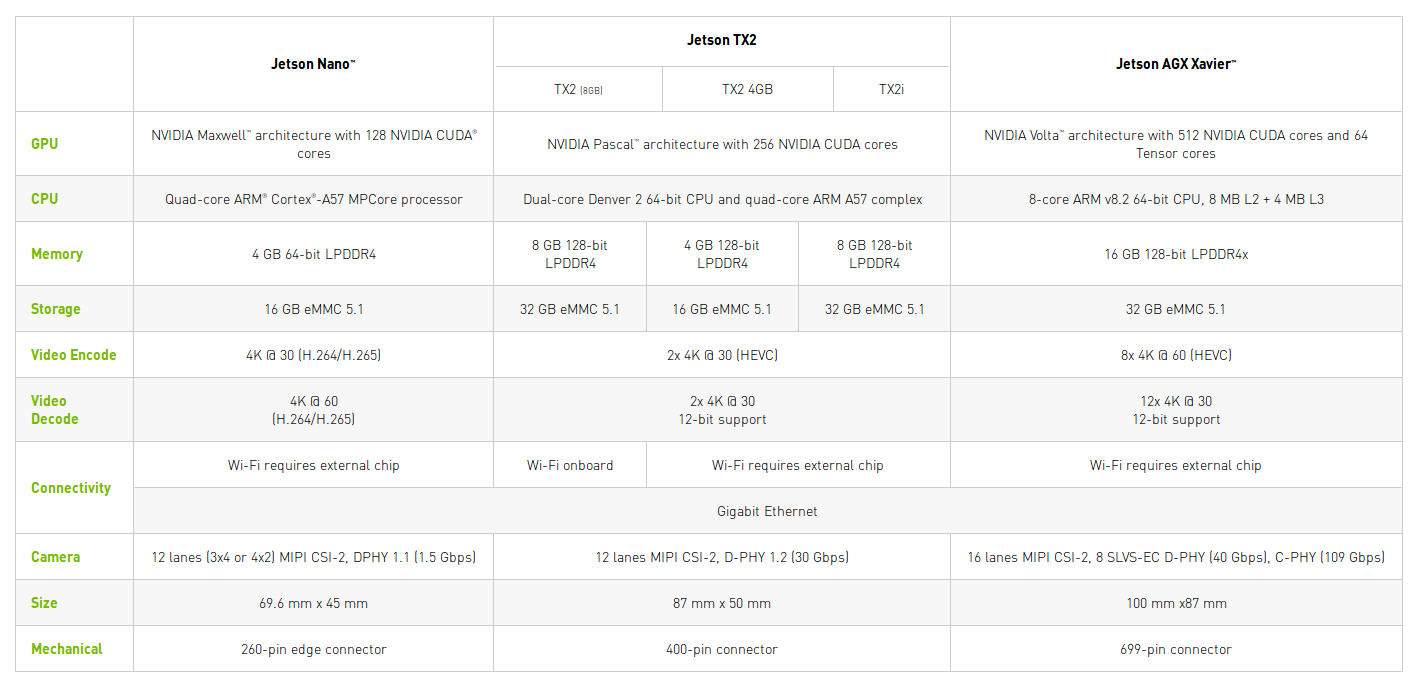
\includegraphics[width=\textwidth]{images/introduction/compare_jetson.png}
\end{figure}
As we can see, unlike other boards Jetson Xavier is build around NVIDIA Volta\texttrademark GPU with tensor cores. These tensor cores accelerate large matrix operations and can perform mixed-precision matrix multiplication and accumulate calculation in a single operation. Each core  provides a 4$\times$4$\times$4 matrix processing array which performs the operation $D = A \cdot B+C$ shown in \ref{tensor_core}, where $A,B,C,D$ are 4$\times$4 matrices. This operation is crucial for most of machine learning applications, especially in deep learning, because, as we will discuss in further chapters, output of each neuron in neural networks are calculated in similar way. 
\begin{figure}[h]
\caption{Tensor core operation https://devblogs.nvidia.com/programming-tensor-cores-cuda-9/}
\label{tensor_core}
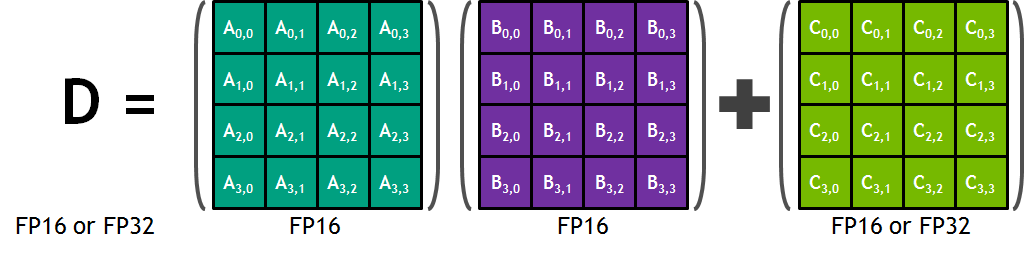
\includegraphics[width=\textwidth]{images/introduction/tensor_core.png}
\end{figure}
Another advantage of Jetson Xavier is using of Nvidia Deep Learning Accelerator engines\footnote{http://nvdla.org/}. These engines improve energy efficiency and free up the GPU to run more complex networks and implemented dynamic tasks  and has up to 5 trillion operations per second (TOPS) INT8 or 2.5 TFLOPS FP16 performance with a power consumption of only 0.5-1.5W. They also supports accelerating of CNN convolution, deconvolution, activation functions, min/max/mean pooling, local response normalization, and fully-connected layers.
\chapter{Related works}
\chapter{Neural networks}
Artificial neural networks are systems inspired by a brain.     The basic computation unit in a brain is a neuron (see \ref{neuron}), which has input and output. The input is a dendritic tree connected to the outputs of other neurons called axons. Neurons operates in a single direction from the input to the output and their output is binary.  
Neurons are also basic computation elements of artificial neural networks. Similarly to biological neural networks, it can have several inputs and outputs. Every neuron can be described by function $f\left(\omega \cdot \textbf{x}  + b\right)$, where $\textbf{x}$ is the input, $\omega$ denotes weights, $b$ is a bias and $f$ is the activation function. 
There are several types of artificial neural networks that are commonly used in machine learning. The most popular type used in object detection is convolutional neural network (CNN), which will be described in the following section.
\begin{figure}[h]
\caption{Neuron cell\cite{staff_2018}}
\label{neuron}
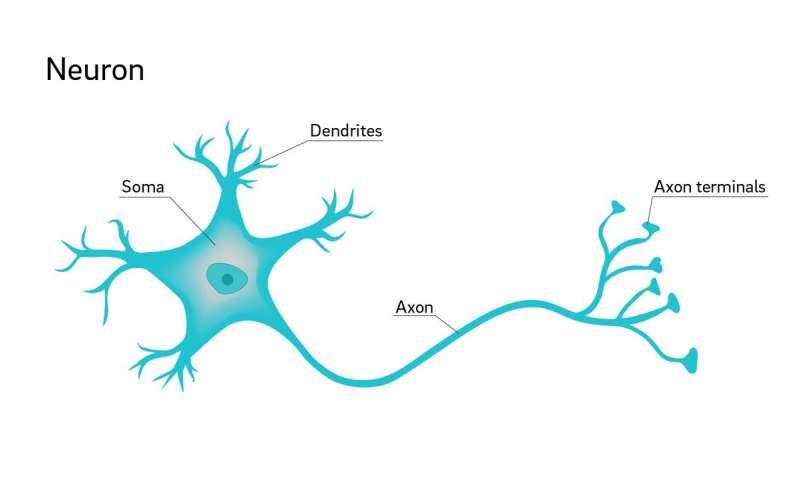
\includegraphics[width=\textwidth]{images/neural_networks/2-whyareneuron.jpg}
\end{figure}
\section{Architecture}
All CNN models has a similar architecture as it is shown in \ref{conv_full}. The input of such neural network is an image. CNN consists of a series of convolution and pooling operations followed by fully connected layers. These operations are described in the next paragraphs. 
\begin{figure}[h]
\caption{Convolutional neural network\cite{britz_2016}}
\label{conv_full}
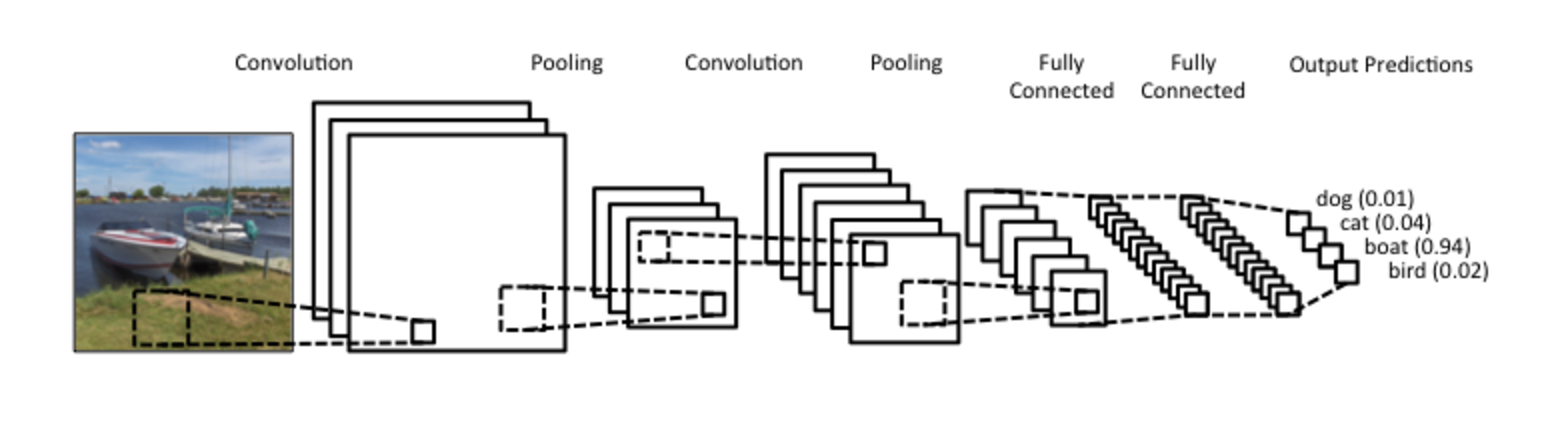
\includegraphics[width=\textwidth]{images/neural_networks/conv_full.png}
\end{figure}
\subsection{Convolutional layer} 
Convolutional layers consist of neurons placed in a grid of size $N \times M \times C$, where $N, M$ denotes width and height of convolutional filter and $C$ is number of channels in the previous layer (see \ref{convolutional_layer}). The filter moves from the left to the right with a certain stride until it completes processing width, then it moves down by the same stride to the beginning of the image    and repeats the process till the whole image is traversed. The process computes convolution as it is shown in \ref{conv_comp}. Calculated feature map is usually smaller than the input, but it is possible to preserve the same dimensionality by using padding to surround the input with zeros. 
\begin{figure}[h]
\caption{Convolutional layer\cite{cs231n}}
\label{convolutional_layer}
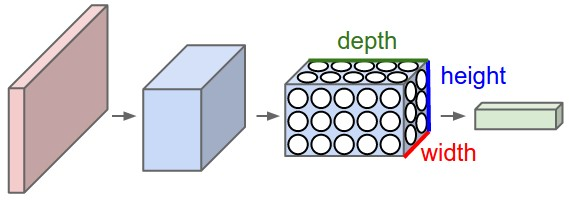
\includegraphics[width=\textwidth]{images/neural_networks/cnn.jpeg}
\end{figure}
\begin{figure}[h]
\caption{Convolution computation\cite{cs231n}}
\label{conv_comp}
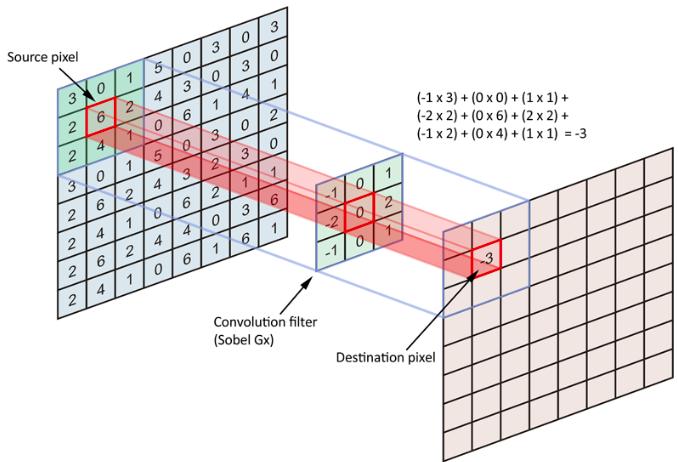
\includegraphics[width=\textwidth]{images/neural_networks/conv.png}
\end{figure}
\subsection{Non-linearity layer}
A non-linearity layer consists of an activation function that takes calculated feature map and creates the activation map as its output. The most common non-linearities used in CNN are sigmoid and ReLu \ref{non-linearity}.
\begin{figure}[h]
\subfloat[ReLu]{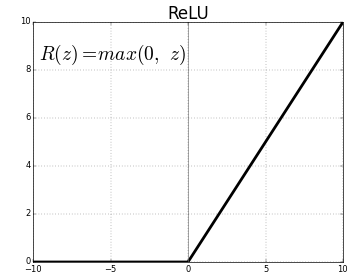
\includegraphics[width=0.6\textwidth]{images/neural_networks/relu.png}}\\
\subfloat[sigmoid]{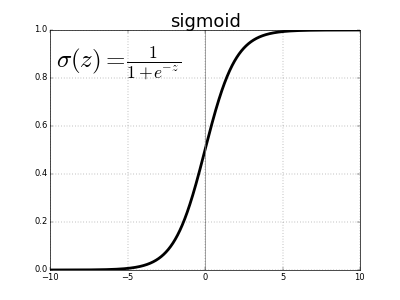
\includegraphics[width=0.68\textwidth]{images/neural_networks/sigmoid.png}}
\caption{Comparation of ReLu and sigmoid non-linearities}
\label{non-linearity}
\end{figure}
\subsection{Pooling layer}
After convolution, pooling layer is used to reduce the dimensionality which enables to reduce number of parameters. Two most common pooling operation are max and min pooling. It simply slides the input with particular stride and choose maximal or minimal value in predefined window (see \ref{pooling}). Pooling helps to not overfit CNN and can reduce the training time.
\begin{figure}[h]
\caption{Pooling layer\cite{cs231n}}
\label{pooling}
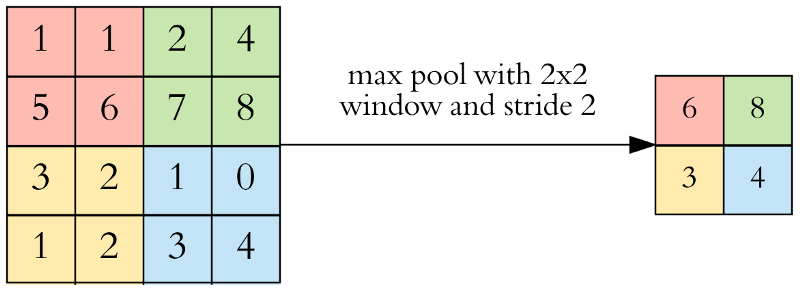
\includegraphics[width=\textwidth]{images/neural_networks/pooling.png}
\end{figure}
\subsection{Fully connected layer}
In fully connected layers, each neuron is connected to every neuron in the previous layer just like in feedforward neural networks.
\section{Training of CNN}
Before we can use any neural network, it must be trained to understand how objects we want it to recognize should look like. The weight of filters are randomized and the filters in lower layers of CNN don't know to look for edges or curves, the filters in higher layers don't know to look for more concrete shapes like wheels, legs, faces. As any supervised learning, CNNs are given a training set of thousands of images with labels to learn features of objects. Learning algorithm is called backpropagation.
\subsection{Backpropagation}
Backpropagation was firstly introduced in\cite{rumelhart_hinton_williams_1986} in 1986. 
This process can be separated into 4 steps: the forward pass, the calculation of loss function, the backward pass and the weight update. During the forward pass, we take a batch of training images and pass it through the network. After first training forward pass output of the network would probably be randomized, because the network isn't able to look for any kind of features, thus isn't able to make any reasonable conclusion about training example.
This goes to the next step of backpropagation, the calculation of loss function.  Each neural network can have its own loss function depending on what its output is, but the most common loss function used for backpropagation is mean squared error
\begin{equation}
L = \frac{1}{2n}\sum_x\norm{y(x) - a(x)}^2      , 
\end{equation}
where $n$ denotes number of training inputs $x$, $y(x)$ label corresponding to the input $x$ and $a$ is network's output.
By training process we want to achieve such a result where the predicted label is the same as the training label. To get this, we want to minimize the amount of loss we have, hence we want to find out which weights most directly contribute to the loss of the networks. This leads to the third step, backward pass, where we calculate partial derivations $\frac{\partial L}{\partial \omega}$, $\frac{\partial L}{\partial b}$. 
Once we compute the derivation, we can update weights and biases by changing them in the opposite direction of the gradient using learning rate $\eta$:
\begin{equation}
\omega = \omega - \eta \frac{\partial L}{\partial \omega}
\end{equation}
\begin{equation}
b = b - \eta \frac{\partial L}{\partial b}
\end{equation}
$\eta$ is the parameter that defines how big steps learning process will take to update the weights, thus how fast we want the model to converge. However, the learning rate that is too big could result in jumps that are too large and not precise enough to reach the optimal point.
Some techniques help to decrease training speed and performance. 
\subsection{Dropout}
Overfitting is one of the biggest problems in machine learning. Overfitting means that a model performs well on a training dataset, but fails on test data. To solve this problem in neural networks, we can use so-called dropout. During each training step, an individual neuron can be dropped out of the net with probability $1 - p$ or kept with probability $p$, so that only a reduced network is trained. The removed neurons are then reinserted into the network with unchanged weights. This methods not only decreases overfitting but also improves training speed. 
\subsection{Batch normalization}
Assume we have a training set of images with cars that has a particular colour. If we try to use the network that was trained on that dataset, it probably will not work well on cars with another colour. In that case, we might need to retrain the network by trying to align the distribution of cars in different colours. Batch normalization https://arxiv.org/pdf/1502.03167.pdf  helps with this problem by reducing the amount of covariance shift in hidden layers. It simply normalizes the output of each layer by subtracting the batch mean and dividing by the batch standard deviation.
After this change of activation output, the weights in the next layer are no longer optimal. Therefore, batch normalization adds two trainable parameters to each layer and lets gradient descent do the denormalization by changing only these parameters during each activation. 
Batch normalization also helps with overfitting, because it adds some noise to each layer's activations. It also allows using higher learning rate, because it makes sure no activation goes high or low. 
\chapter{Used networks}
\section{ResNet}
Residual networks described in \cite{he_zhang_ren_sun_2016} are classification networks with an image as the input and object class and confidence score as the output. In this paper, they introduced shortcut connections that are widely used in modern neural networks.  One of the biggest problems with training deep neural networks is vanishing and exploding gradient. During backpropagation, a lot of small or large numbers are multiplied to compute gradients. When the network is deep, multiplying of small numbers will become zero (vanished) and multiplying of large numbers will explode. Normally we expect deeper neural network will have more accurate predictions, but the opposite is true, and this degradation problem is caused by the vanishing gradient.
This problem can be solved by adding shortcut connection which adds the input to the output after few weight layers, hence the output is $H(x) = F(x) + x$ (see \ref{resnet_block}). 
There are two types of residual connections. The identity shortcuts can be directly used when both input and output have the same dimension, or extra zero padding can be used when dimensions change. In both cases, no extra parameters are needed. 
Comparing plain and residual network with 34 layers (see \ref{resnet}) Top-1 error drops from 28.54\% to 25.03\%. On the other hand, if we compare smaller network with 18 layers, Top-1 error changes from 27.94\% to 27.88\%, which means shortcut connections perform better in deeper networks. 
\begin{figure}[h]
\caption{Residual block}
\label{resnet_block}
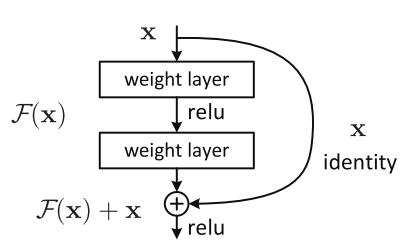
\includegraphics[width=.5\textwidth]{images/used_networks/resnet_block.png}
\end{figure}
\begin{figure}[h]
\caption{ResNet architecture}
\label{resnet}
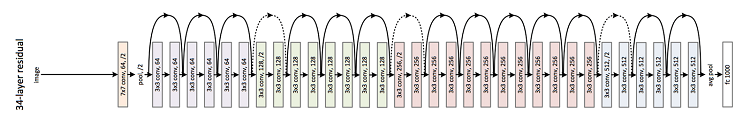
\includegraphics[width=\textwidth]{images/used_networks/resnet.png}
\end{figure}
ResNets with different number of layers are often used as classification networks (backbone) in detectors such as RetinaNet.  
\section{RetinaNet}
https://medium.com/@14prakash/the-intuition-behind-retinanet-eb636755607d
RetinaNet was proposed by Facebook AI Research and its features are described in \cite{lin_dollar_girshick_he_hariharan_belongie_2017} and \cite{lin_goyal_girshick_he_dollar_2017}. 
They proposed using anchor boxes instead of predicting bounding boxes. Sizes of the anchor boxes are predefined and used in further predictions. Thus, the network does not predict the final size of the object, but instead, it only adjusts the size of the nearest anchor to the size of the object. 
Also, they suggested a solution for object detection in different scales. Originally a pyramid of the same image at different scales was used to detect the object. However, this solution is time-consuming and has a high memory demand. Instead, a pyramid of features can be used. Although it is not such efficient for accurate object detection as image pyramids, it provides result faster and with less memory consumption. In \cite{lin_dollar_girshick_he_hariharan_belongie_2017} authors propose Feature Pyramid Network (FPN) which is fast like the described pyramid of features, but more accurate. Its architecture is seen in \ref{fpn}.
The other solution, focal loss, solves class imbalance. Instead of normal cross entropy calculated by 
\begin{equation}
C(p, y) = -\sum_{i}y_i \ln p_i
\end{equation}  
scaled entropy is used using following equation:
\begin{equation}
C(p,y)=-\sum_i y_i(1-p_i)^{\lambda}\ln p_i.
\end{equation}
Here we can see focusing parameter $\lambda \geq 0$ which smoothly adjusts the rate at which easy examples are down weighted and thus training is focused on hard negatives. 
\begin{figure}[h]
\caption{Feature Pyramid Network}
\label{fpn}
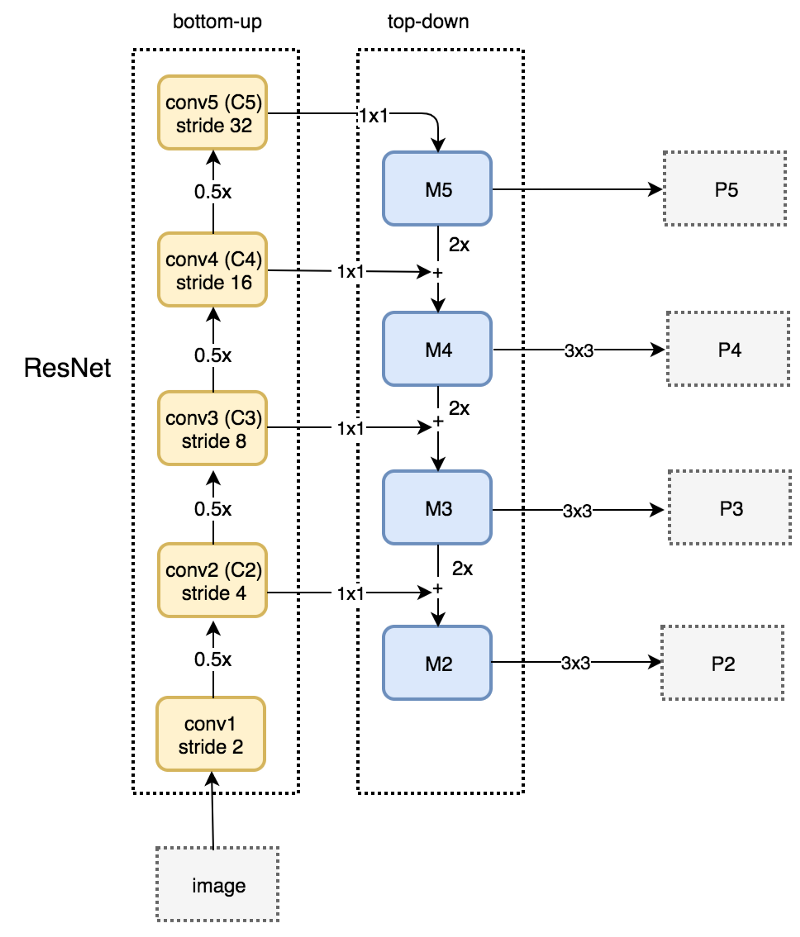
\includegraphics[width=\textwidth]{images/used_networks/fpn.png}
\end{figure}
In this thesis we used Keras implementation of RetinaNet\footnote{https://github.com/fizyr/keras-retinanet} implemented in $TensorFlow$ with ResNet50 as a backbone. 
\section{SqueezeDet}
SqueezeDet (https://arxiv.org/pdf/1612.01051.pdf) is a single stage detection pipeline inspired by YOLO. The main difference between two architectures is that SqueezeDet uses SqueezeNet (https://arxiv.org/pdf/1602.07360.pdf) for feature extraction.
The building brick of SqueezeNet is called fire module \ref{fire_squeezenet}. Each fire module contains a squeeze layer and an expand layer. Squeeze layers replace 3$\times$3 filters by 1$\times$1 filters to reduce computation complexity 9 times. Following expand layers contain number of 1$\times$1  and 3$\times$3 kernels.    Squeeze layers reduce depth of calculated feature map, which means the following 3$\times$3 filters in expand layers have to do fewer computation. Thanks to its architecture, SqueezeDet can be faster and smaller comparing to other state-of-art solutions (see \ref{squeezedet_comparasion}), and so can be efficiently used on embedded system. 
\begin{figure}[h]
\caption{Fire module in SqueezeNet}
\label{fire_squeezenet}
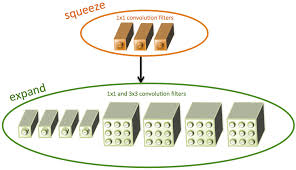
\includegraphics[width=.5\textwidth]{images/used_networks/fire_squeezenet.jpeg}
\end{figure}
\begin{figure}[h]
\caption{SqueezeDet comparison with other state-of-art solutions}
\label{squeezedet_comparasion}
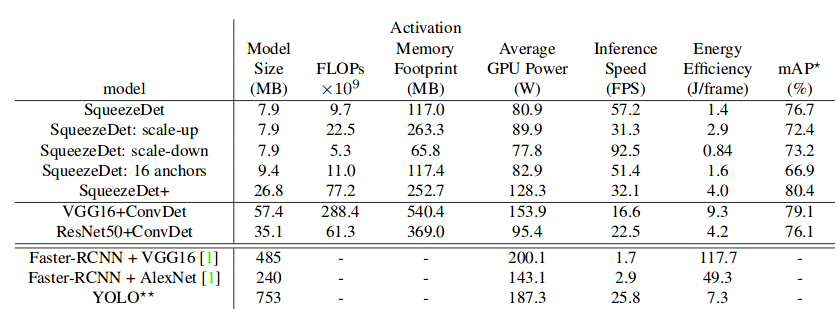
\includegraphics[width=\textwidth]{images/used_networks/squeezedet_comparation.png}
\end{figure}
The loss function of SqueezeDet is defined as
\begin{multline}
\frac{\lambda_{bbox}}{N_{obj}}\sum_{i=1}^W\sum_{j=1}^H\sum_{k=1}^KI_{ijk}\left[\left(\beta x_{ijk}-\beta x_{ijk}^G\right)^2+\left(\beta y_{ijk} - \beta y_{ijk}^G\right)^2\right. \\
+\left(\beta w_{ijk}-\beta w_{ijk}^G\right)^2 + \left(\beta h_{ijk}-\beta h_{ijk}^G\right)^2\left. \right]\\
+\sum_{i=1}^W\sum_{j=1}^H\sum_{k=1}^K\frac{\lambda^{+}_{conf}}{N_{obj}}I_{ijk}\left(\gamma_{ijk}-\gamma_{ijk}^G\right)^2 + \frac{\lambda^{-}_{conf}}{WHK-N_{obj}}\bar{I}_{ijk}\gamma^2_{ijk}\\
+\frac{1}{N_{obj}}\sum_{i=1}^W\sum_{j=1}^H\sum_{k=1}^K\sum_{c=1}^CI_{ijk}l_c^G\log(p_c)
\end{multline},
where first part is the bounding box regression and $\left(\beta x_{ijk}, \beta y_{ijk}, \beta w_{ijk}, \beta h_{ijk}\right)$ corresponds to the relative coordinate of anchor-$k$ located at grid center-$(i,j)$. Second part denotes confidence score regression with output $\gamma_{ijk}$. The last part is cross-entropy   loss for classification.
We used a tensorflow implementation of SqueezeDet available to download from GitHub\footnote{https://github.com/BichenWuUCB/squeezeDet}.
\section{YOLO}
\subsection{YOLO v1}
A new approach for object detection, YOLO architecture, was presented in \cite{redmon_divvala_girshick_farhadi_2016}. A single neural network is used to predict both bounding boxes and class probabilities, hence an image is evaluated only once. The described system divides the input into a $S \times S$ grid, and if the center of an object falls into a grid cell, this cell is responsible for detecting that object. Each cell also predicts $B$ bounding boxes and confidence score for them. Confidence is defined as 
\begin{equation}
score = Pr(Object)\cdot IoU^{truth}_{pred},
\end{equation}
where $Pr(Object)$ is a probability of an object being inside that bounding box and $IoU^{truth}_{pred}$ denotes intersection over union between ground truth and prediction. 
Each bounding box consists of $\left(x, y, w, h, score\right)$, where $\left(x, y\right)$ represents the center of the box and $\left(w, h\right)$ denotes its width and height. Each grid cells also predicts conditional probability $C = Pr(Class_i|Object)$.
The model consists of 24 convolutional layers followed by 2 fully connected layers as it is shows in \ref{yolov1}.
\begin{figure}[h]
\caption{YOLO v1 architecture}
\label{yolov1}
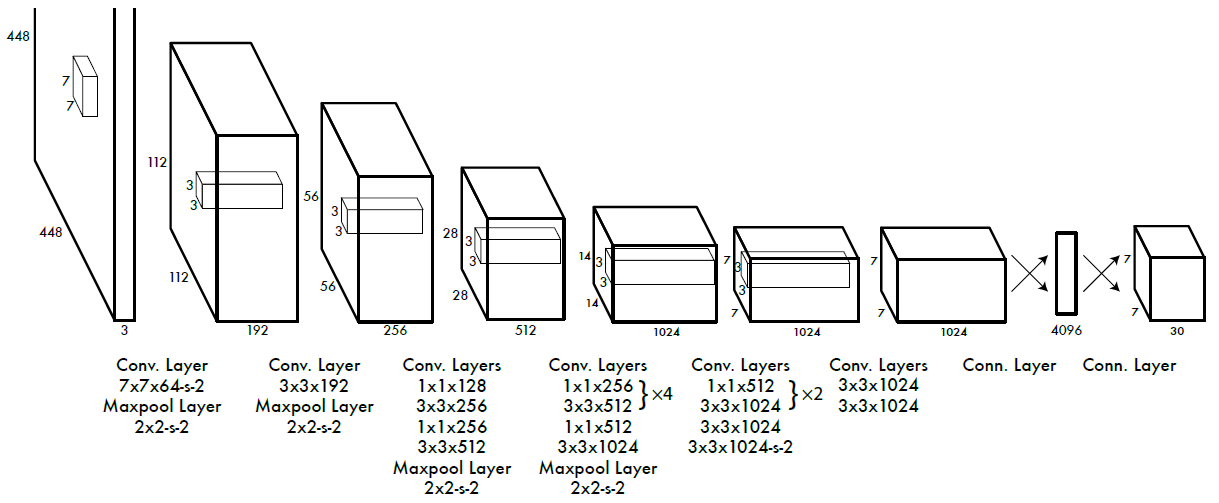
\includegraphics[width=\textwidth]{images/used_networks/yolov1.png}
\end{figure}
Training process optimizes loss function
\begin{multline}
\lambda_{coord}\sum_{i=0}^{S^2}\sum_{j=0}^{B}\textbf{1}_{ij}^{obj}\left[\left(x_i - \hat{x}_i\right)^2+\left(y_i + \hat{y}_i\right)^2\right]\\
+\lambda_{coord}\sum_{i=0}^{S^2}\sum_{j=0}^{B}\textbf{1}_{ij}^{obj}\left[\left(\sqrt{w_i} - \sqrt{\hat{w_i}}\right)^2+\left(\sqrt{h_i} + \sqrt{\hat{h}_i}\right)^2\right]\\
+\sum_{i=0}^{S^2}\sum_{j=0}^{B}\textbf{1}_{ij}^{obj}\left(C_i-\hat{C}_i\right)^2\\
+\lambda_{noobj}\sum_{i=0}^{S^2}\sum_{j=0}^{B}\textbf{1}_{ij}^{noobj}\left(C_i-\hat{C}_i\right)^2\\
+\sum_{i=0}^{S^2}\textbf{1}_{ij}^{obj}\sum_{c\in classes}\left(p_i(c) - \hat{p}_i(c)\right)^2
\end{multline},
where 
\begin{equation}
  \textbf{1}_{ij}^{obj}=\begin{cases}
    1, & \text{if there is an object}.\\
    0, & \text{otherwise},
  \end{cases}
\end{equation}
$\textbf{1}_{ij}^{noobj}$ is inverse function to $\textbf{1}_{ij}^{obj}$, $\lambda_{coord}$ and $\lambda_{noobj}$ are constant to increase the loss from bounding box coordinate prediction and decrease the loss from confidence prediction for boxes that does not contain objects. 
While YOLO v1 was faster than most of the existing approaches for object detection, it had relatively low 57.9\% mAP on the VOC 2012 test set compared to the existing state of the art. 
\subsection{YOLO v2}
A new version of YOLO was introduced in \cite{redmon_farhadi_2017}. Authors of this state of the art detector refer to it as a better, faster and stronger version of YOLO. For better performance, they added batch normalization and used images with a bigger resolution to train the network. They also removed fully connected layers and used anchor boxes to predict bounding boxes, which lead to a small decrease in mAP from 69.5\% to 69.2\%, but it also increased a recall from 81\% to 88\%. We can see how applied changes improved network performance in \ref{yolov2_improve}.
\begin{figure}[h]
\caption{YOLO v2 improvement}
\label{yolov2_improve}
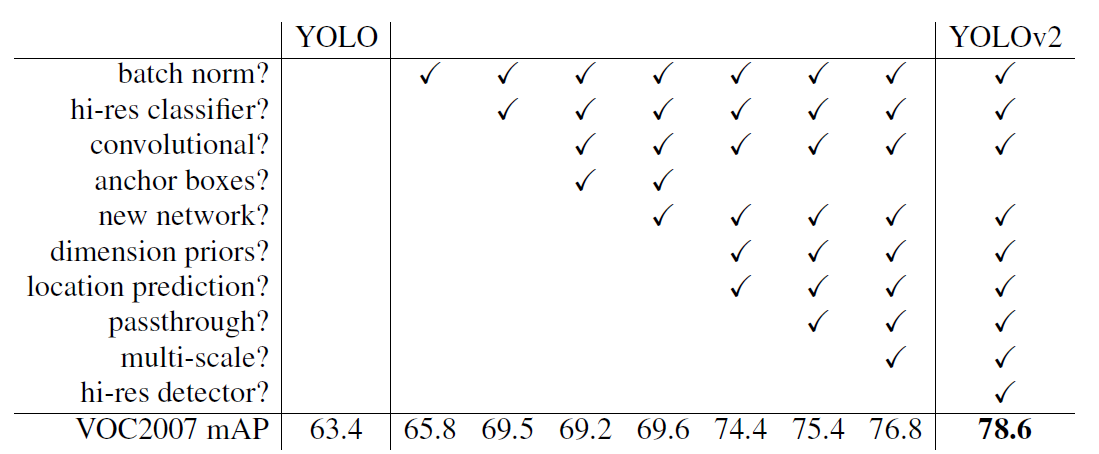
\includegraphics[width=\textwidth]{images/used_networks/yolov2_improve.png}
\end{figure}
They also proposed a new classification network called Darknet-19 (see Appendix \ref{darknet-19}) to make YOLO even faster. We can see that Darknet-19 has many $1\times 1$ convolutions to reduce the number of parameters. 

\subsection{YOLO v3}
The newest version of YOLO was presented in \cite{Redmon2018YOLOv3AI}. Similar to YOLOv2 it predicts bounding boxes using dimension clusters as anchor boxes. The network predicts four coordinates for each bounding box and for training they use a sum of squared error loss. Objectness score for each bounding box is predicted using logistic regression, which should be one if the bounding box prior overlaps a ground truth object by more than any other bounding box prior. 
They also use 3 different scales for prediction, which is similar to feature pyramid networks. Deeper extractor called Darknet-53 (see Appendix \ref{darknet-53}) with shortcut connections is used for feature extraction.

Comparing to other state of art solutions, YOLO v3 has similar performance, but it is much faster as it is seen in \ref{yolov3-compare}.
Unlike RetinaNet and SqueezeDet, YOLO uses another neural network framework, Darknet\footnote{https://pjreddie.com/darknet/}, written in C and CUDA. 
\begin{figure}[h]
\caption{YOLO v3 comparation}
\label{yolov3-compare}
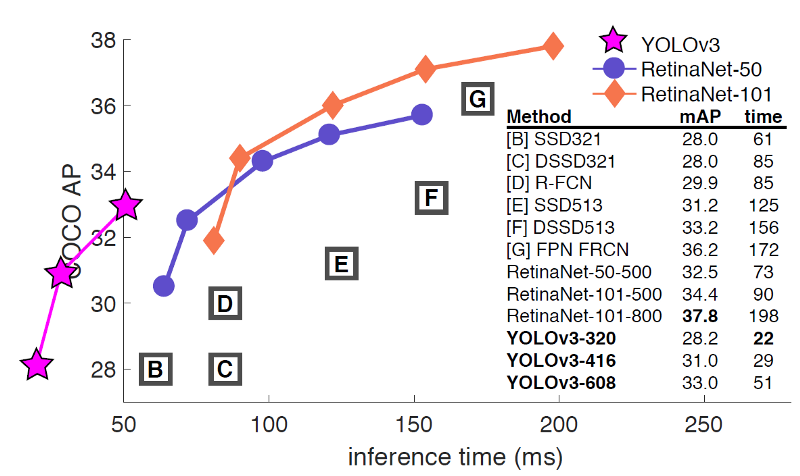
\includegraphics[width=\textwidth]{images/used_networks/yolov3_comparasion.png}
\end{figure}
\chapter{Experiments}
For experiments, we chose SqueezeDet, YOLOv3, and RetinaNet. We trained all three networks on KITTI (http://www.cvlibs.net/datasets/kitti/) and internal GoodVision dataset specifically prepared for our use case. Thanks to the ability of RetinaNet and YOLOv3 to adapt to the size of the input image, we were able to test different image size ratios with no need to retrain these networks.  YOLOv3 was evaluated with two different input image resolutions: 608$\times$608 and 418$\times$418; for evaluation of RetinaNet, we used three different largest side sizes: 1024, 608 and 418. Unfortunately, SqueezeDet does not adapt its layers to an input image, so we used a network with input image resolution 1242$\times$375 defined by the pre-trained model.
\section{Datasets}
\subsection{KITTI dataset}
KITTI dataset consists of 7481 training images and 7518 test images with a total of 80256 labeled objects. Original datasets has 9 different type of objects: ``Car'', ``Van'', ``Truck'', ``Pedestrian'', ``Person\_sitting'', ``Cyclist'', ``Tram'', ``Misc'' or ``DontCare''. We used only 5 of them for training: ``Car'', ``Van'', ``Truck'', ``Pedestrian'', ``Person\_sitting'', though we merged ``Person\_sitting'' and ``Pedestrian'' classes into single ``Person'' object type. Regardless   of lack of common classes like ``Bus'', ``Bicycle'', ``Motorcycle'', it fits our needs, because all data were gathered by driving around cities, in country areas, and on highways, and so out networks would be trained on real-life traffic data with no redundant information \ref{fig:kitti-examples}.       
\begin{figure}[hbt]
        \centering
        \subfloat{
                \centering
                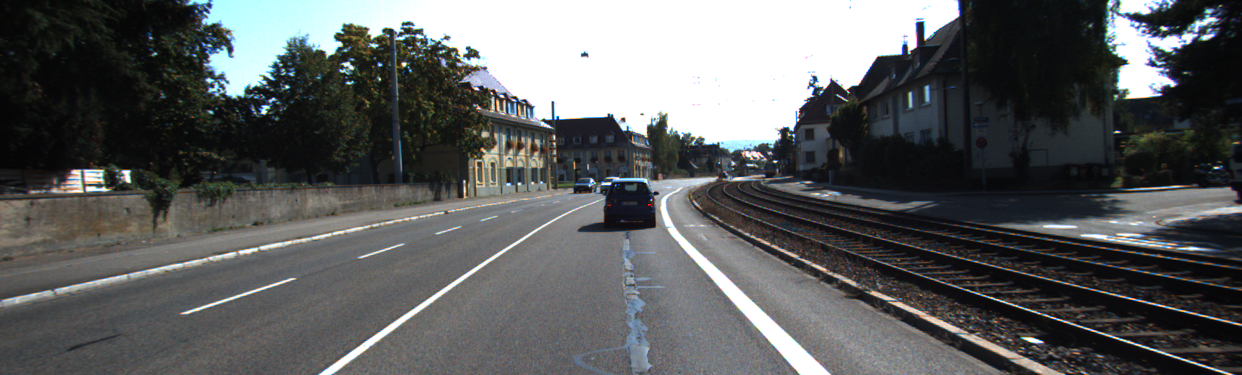
\includegraphics[width=\linewidth]{images/experiments/kitti-1.png}\label{fig:kitti-1}
        }
        
        \hfill
        \subfloat{
                \centering
                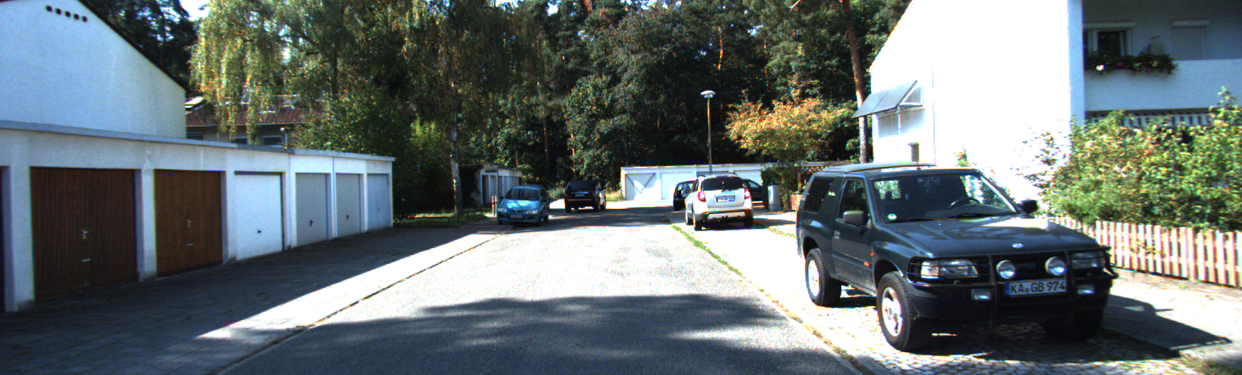
\includegraphics[width=\linewidth]{images/experiments/kitti-2.png}\label{fig:kitti-1}
        }
                \caption{Image samples from KITTI dataset}
                \label{fig:kitti-examples}
\end{figure}
\subsection{GoodVision dataset}
Internal GoodVision dataset was specifically created for object detection and recognition in traffic. It consists of 4917 images with more than 130000 labeled objects. Unlike in KITTI dataset, such classes as ``Bicycle'', ``Bus'', ``Motorcycle'' are presented here, which means neural networks trained on this dataset will be more complex and more adequate for our use case.  Images for this dataset were gathered from cameras placed at different heights and angles to roads and highways. Samples from the dataset are presented in \ref{fig:goodvision-samples}.

\begin{figure}[hbt]
        \centering
        \subfloat{
                \centering
                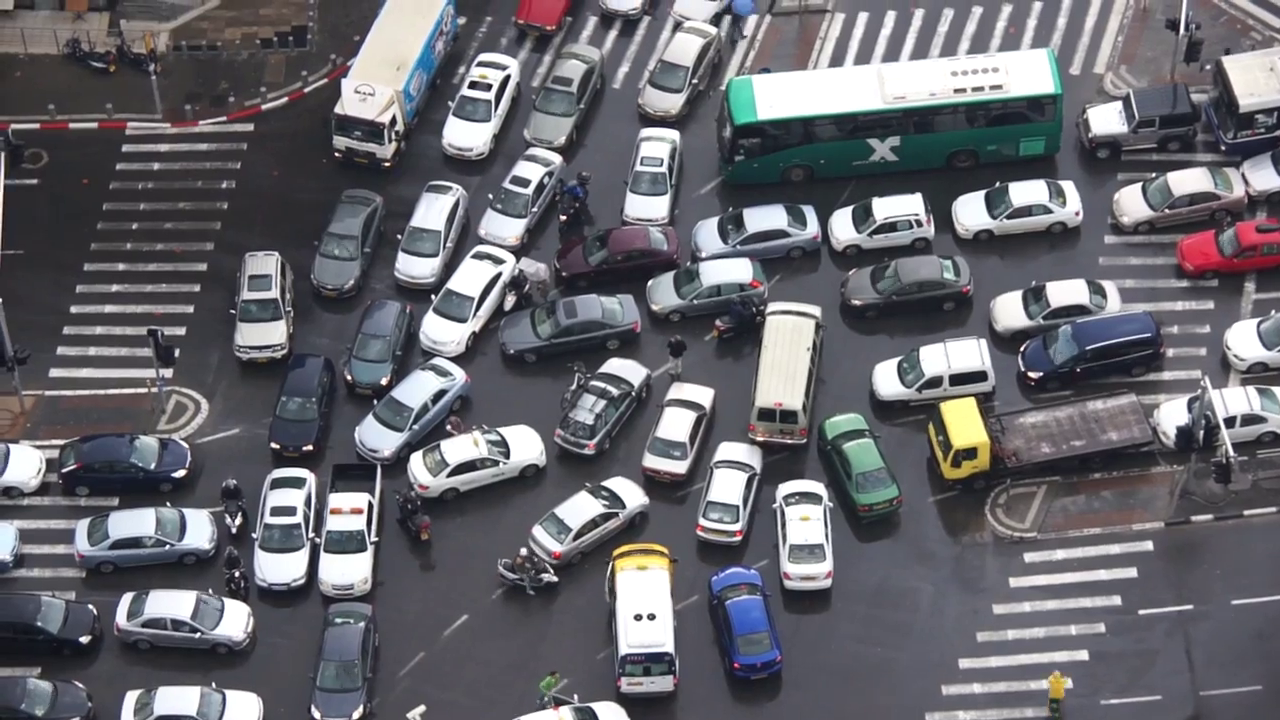
\includegraphics[width=.8\linewidth]{images/experiments/gv1.png}\label{fig:gv2}
        }
        
        \centering
        \subfloat{
                \centering
                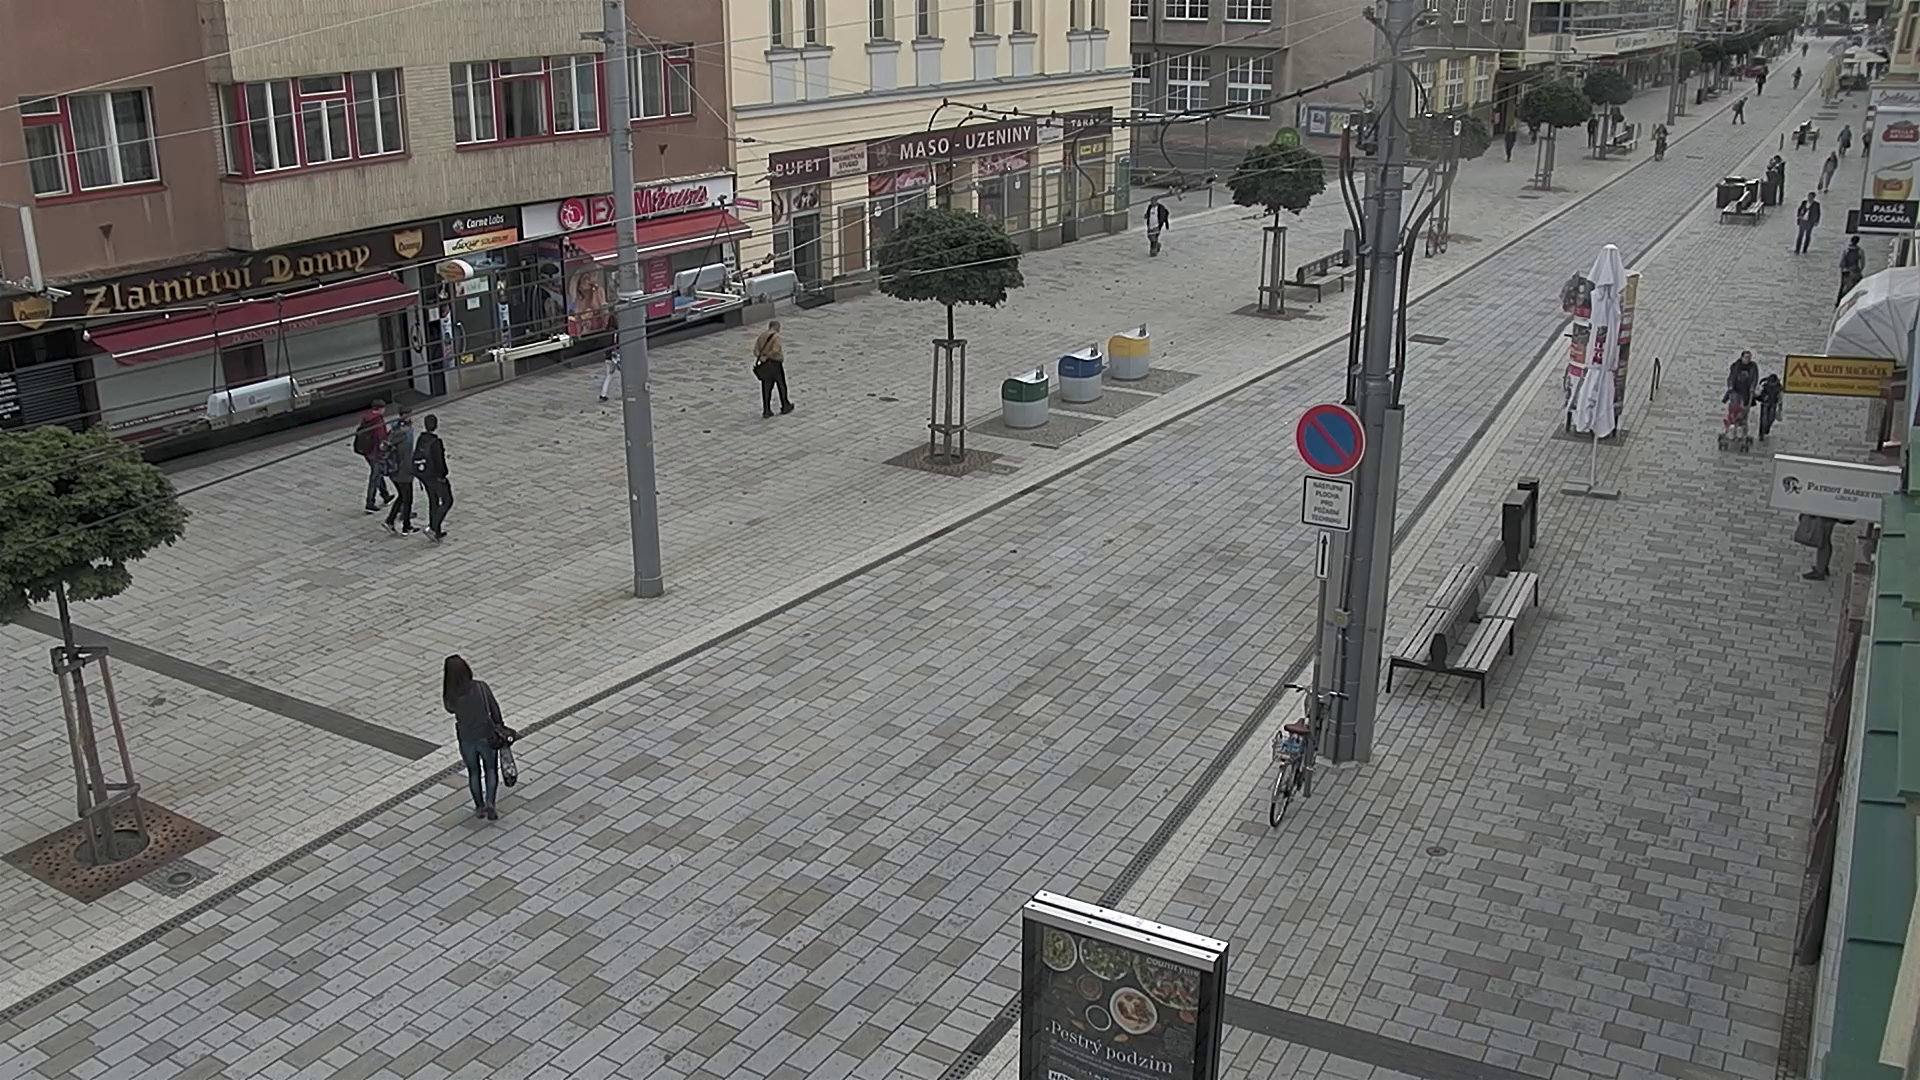
\includegraphics[width=.8\linewidth]{images/experiments/gv2.png}\label{fig:gv1}
        }
                \caption{Image samples from GoodVision dataset}
                \label{fig:goodvision-samples}
\end{figure}
\section{Performance evaluation}
For our evaluation, we calculated average precision for every class in the evaluation set. We had to calculate precision and recall, which are defined as
\begin{equation}
Precision = \frac{TP}{TP+FP},
\end{equation}
\begin{equation}
Recall = \frac{TP}{TP+FN},
\end{equation}
where TP is true positives, FP is false positives, and FN is false negatives.
It means precision measures how accurate predictions are, while recall refers to the percentage of total relevant results correctly classified by our network.
To determine if the prediction is a true positive or a false positive, intersection over union (IoU) has to be measured. As picture \ref{iou} shows, IoU is simply the ratio between the area of overlap between the ground truth bounding box and predicted bounding box, and the area encompassed by both ground truth bounding box and predicted bounding box. If IoU is over some predefined threshold, the prediction is considered to be true. Otherwise, it is a false positive. For evaluation, we chose this threshold to be 0.5.
Then we calculate precision/recall curve (https://acutecaretesting.org/en/articles/precision-recall-curves-what-are-they-and-how-are-they-used) and average precision is area under that curve and is calculated for every class independently. Mean average precision is simply average value of average precisions across all classes. 
\begin{figure}[h]
\caption{Intersection over Union https://www.pyimagesearch.com/2016/11/07/intersection-over-union-iou-for-object-detection/}
\label{iou}
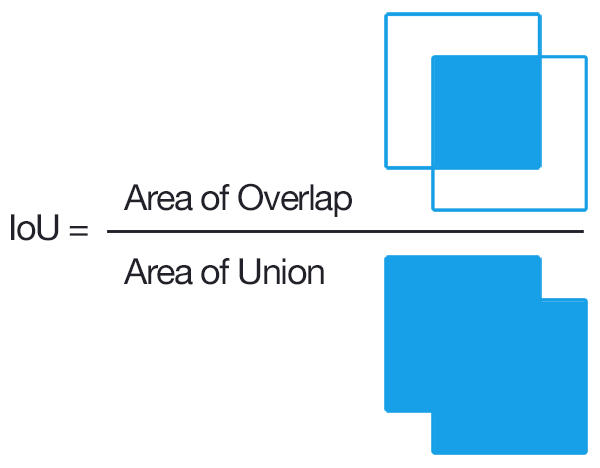
\includegraphics[width=.4\textwidth]{images/experiments/iou_equation.png}
\end{figure}
Results of the evaluation are presented in table \ref{tab:cnn_evaluation}. YOLOv3 performs better than both SqueezeDet and RetinaNet at both resolution. Although YOLOv3 trained on KITTI dataset indicates bigger mAP on KITTI evaluation set, it has worse performance on GoodVision evaluation set, while YOLOv3 trained on GoodVision dataset has almost 10\% better mAP. We can notice this trend for all 3 CNNs: while KITTI-trained model has better performance on KITTI test set, it fails on GoodVision set. If we compare models trained on KITTI and GoodVision dataset using AP of classes presented in KITTI dataset only, the difference will be even bigger. 
% Please add the following required packages to your document preamble:
% \usepackage{multirow}
% \usepackage[table,xcdraw]{xcolor}
% If you use beamer only pass "xcolor=table" option, i.e. \documentclass[xcolor=table]{beamer}
\begin{table}[hbt]
\renewcommand{\arraystretch}{2.5}
\catcode`\-=12
\resizebox{\textwidth}{!}{
\begin{tabular}{|c|c|c|c|c|c|c|c|c|c|c|}
\hline
\cellcolor[HTML]{C0C0C0}                                 & \cellcolor[HTML]{C0C0C0}                                            & \cellcolor[HTML]{C0C0C0}                                           & \cellcolor[HTML]{C0C0C0}                                               & \cellcolor[HTML]{C0C0C0}                                           & \cellcolor[HTML]{C0C0C0}                                                  & \cellcolor[HTML]{C0C0C0}                                           & \cellcolor[HTML]{C0C0C0}                                              & \cellcolor[HTML]{C0C0C0}                                             & \cellcolor[HTML]{C0C0C0}                                           & \cellcolor[HTML]{C0C0C0}                                        \\
\multirow{-2}{*}{\cellcolor[HTML]{C0C0C0}\textbf{Model}} & \multirow{-2}{*}{\cellcolor[HTML]{C0C0C0}\textbf{Training dataset}} & \multirow{-2}{*}{\cellcolor[HTML]{C0C0C0}\textbf{Testing dataset}} & \multirow{-2}{*}{\cellcolor[HTML]{C0C0C0}\textbf{Bicycle AP {[}\%{]}}} & \multirow{-2}{*}{\cellcolor[HTML]{C0C0C0}\textbf{Bus AP {[}\%{]}}} & \multirow{-2}{*}{\cellcolor[HTML]{C0C0C0}\textbf{Motorcycle AP {[}\%{]}}} & \multirow{-2}{*}{\cellcolor[HTML]{C0C0C0}\textbf{Car AP {[}\%{]}}} & \multirow{-2}{*}{\cellcolor[HTML]{C0C0C0}\textbf{Person AP {[}\%{]}}} & \multirow{-2}{*}{\cellcolor[HTML]{C0C0C0}\textbf{Truck AP {[}\%{]}}} & \multirow{-2}{*}{\cellcolor[HTML]{C0C0C0}\textbf{Van AP {[}\%{]}}} & \multirow{-2}{*}{\cellcolor[HTML]{C0C0C0}\textbf{mAP {[}\%{]}}} \\ \hline
                                                         & GoodVision                                                          & GoodVision                                                         & 62,5                                                                   & 72,4                                                               & 54,4                                                                      & 89,3                                                               & 91,2                                                                  & 83,2                                                                 & 80,1                                                               & 76,2                                                            \\ \cline{2-11} 
                                                         &                                                                     & KITTI                                                              & --                                                                     & --                                                                 & --                                                                        & 81,4                                                               & 89,3                                                                  & 80,6                                                                 & 73,5                                                               & 81,2                                                            \\ \cline{3-11} 
\multirow{-3}{*}{YOLOv3 608}                             & \multirow{-2}{*}{KITTI}                                             & GoodVision                                                         & --                                                                     & --                                                                 & --                                                                        & 58,6                                                               & 72,3                                                                  & 73,2                                                                 & 67,0                                                               & 67,8                                                            \\ \hline
                                                         & GoodVision                                                          & GoodVision                                                         & 63,6                                                                   & 61,2                                                               & 40,7                                                                      & 83,4                                                               & 84,0                                                                  & 72,7                                                                 & 65,2                                                               & 67,3                                                            \\ \cline{2-11} 
                                                         &                                                                     & KITTI                                                              & --                                                                     & --                                                                 & --                                                                        & 73,6                                                               & 80,7                                                                  & 68,3                                                                 & 59,5                                                               & 70,5                                                            \\ \cline{3-11} 
\multirow{-3}{*}{YOLOv3 416}                             & \multirow{-2}{*}{KITTI}                                             & GoodVision                                                         & --                                                                     & --                                                                 & --                                                                        & 52,1                                                               & 63,5                                                                  & 62,2                                                                 & 43,0                                                               & 55,2                                                            \\ \hline
                                                         & GoodVision                                                          & GoodVision                                                         & 46,3                                                                   & 34,8                                                               & 15,4                                                                      & 39,5                                                               & 32,3                                                                  & 53,8                                                                 & 40,6                                                               & 37,5                                                            \\ \cline{2-11} 
                                                         &                                                                     & KITTI                                                              & --                                                                     & --                                                                 & --                                                                        & 35,2                                                               & 29,9                                                                  & 51,6                                                                 & 31,1                                                               & 37,0                                                            \\ \cline{3-11} 
\multirow{-3}{*}{RetinaNet 1024}                         & \multirow{-2}{*}{KITTI}                                             & GoodVision                                                         & --                                                                     & --                                                                 & --                                                                        & 20,6                                                               & 23,3                                                                  & 42,2                                                                 & 19,4                                                               & 26,4                                                            \\ \hline
                                                         & GoodVision                                                          & GoodVision                                                         & 11,0                                                                   & 12,7                                                               & 0,2                                                                       & 25,5                                                               & 18,0                                                                  & 28,3                                                                 & 23,4                                                               & 17,0                                                            \\ \cline{2-11} 
                                                         &                                                                     & KITTI                                                              & --                                                                     & --                                                                 & --                                                                        & 23,0                                                               & 16,6                                                                  & 27,8                                                                 & 20,3                                                               & 21,9                                                            \\ \cline{3-11} 
\multirow{-3}{*}{RetinaNet 608}                          & \multirow{-2}{*}{KITTI}                                             & GoodVision                                                         & --                                                                     & --                                                                 & --                                                                        & 2,3                                                                & 16,3                                                                  & 24,6                                                                 & 18,1                                                               & 15,3                                                            \\ \hline
                                                         & GoodVision                                                          & GoodVision                                                         & 0,0                                                                    & 5,8                                                                & 0,6                                                                       & 19,5                                                               & 12,9                                                                  & 15,8                                                                 & 16,7                                                               & 10,2                                                            \\ \cline{2-11} 
                                                         &                                                                     & KITTI                                                              & --                                                                     & --                                                                 & --                                                                        & 19,1                                                               & 12,3                                                                  & 14,6                                                                 & 15,1                                                               & 15,3                                                            \\ \cline{3-11} 
\multirow{-3}{*}{RetinaNet 416}                          & \multirow{-2}{*}{KITTI}                                             & GoodVision                                                         & --                                                                     & --                                                                 & --                                                                        & 13,4                                                               & 7,8                                                                   & 10,6                                                                 & 11,2                                                               & 10,8                                                            \\ \hline
                                                         & GoodVision                                                          & GoodVision                                                         & 1,7                                                                    & 8,2                                                                & 4,1                                                                       & 34,4                                                               & 39,2                                                                  & 22,9                                                                 & 12,9                                                               & 17,6                                                            \\ \cline{2-11} 
                                                         &                                                                     & KITTI                                                              & --                                                                     & --                                                                 & --                                                                        & 30,6                                                               & 38,5                                                                  & 22,5                                                                 & 10,8                                                               & 25,6                                                            \\ \cline{3-11} 
\multirow{-3}{*}{squeezeDet}                             & \multirow{-2}{*}{KITTI}                                             & GoodVision                                                         & --                                                                     & --                                                                 & --                                                                        & 3,1                                                                & 2,9                                                                   & 4,7                                                                  & 4,2                                                                & 3,7                                                             \\ \hline
\end{tabular}
}
\caption{CNN evaluation}
\label{tab:cnn_evaluation}
\end{table}
\section{Inference time evaluation}
For computing on the edge, we should ensure that time delay between receiving input data, in this case stream frame,  and providing output data to a user is as small as possible. Time of object detection and classification can be the biggest bottleneck in such systems, therefore it is necessary to choose such architecture that provides the best result with the least possible inference time. 
Videos for this evaluation were taken from video databases with free access such as YouTube or Pexels. All videos have different camera view with various object count, video resolution and FPS, as shown in table \ref{video_characteristics}. This can affect neural network detector performance, hence we should also compare various input resolutions of neural networks. Video samples presented in \ref{fig:samples} shows obvious difference between videos scenes. Those scenes represents typical use case for our system.
% Please add the following required packages to your document preamble:
% \usepackage{multirow}
% \usepackage[table,xcdraw]{xcolor}
% If you use beamer only pass "xcolor=table" option, i.e. \documentclass[xcolor=table]{beamer}
\begin{table}[htb]
\resizebox{\textwidth}{!}{
\begin{tabular}{|c|c|c|}
\hline
\cellcolor[HTML]{C0C0C0}                                                              & \cellcolor[HTML]{C0C0C0}{\color[HTML]{333333} }                               & \cellcolor[HTML]{C0C0C0}                                            \\
\cellcolor[HTML]{C0C0C0}                                                              & \cellcolor[HTML]{C0C0C0}{\color[HTML]{333333} }                               & \cellcolor[HTML]{C0C0C0}                                            \\
\multirow{-3}{*}{\cellcolor[HTML]{C0C0C0}\textbf{Video file}}                         & \multirow{-3}{*}{\cellcolor[HTML]{C0C0C0}{\color[HTML]{333333} \textbf{FPS}}} & \multirow{-3}{*}{\cellcolor[HTML]{C0C0C0}\textbf{Video Resolution}} \\ \hline
5.4 4K Camera Road in Thailand.mp4                                                    & 30                                                                            & 1280x720                                                            \\ \hline
Cars Driving On Street.mp4                                                            & 30                                                                            & 1920x1080                                                           \\ \hline
Cars On Highway.mp4                                                                   & 25                                                                            & 1920x1080                                                           \\ \hline
Cars On The Road.mp4                                                                  & 50                                                                            & 1280x720                                                            \\ \hline
City Traffic.mp4                                                                      & 30                                                                            & 1920x1088                                                           \\ \hline
Day Traffic Sample Video Dataset.mp4                                                  & 30                                                                            & 432x240                                                             \\ \hline
Pedestrian and Traffic, Human Activity Recognition Video ,DataSet By UET Peshawar.mp4 & 30                                                                            & 1280x720                                                            \\ \hline
Pexels Videos 1601538.mp4                                                             & 25                                                                            & 1920x1080                                                           \\ \hline
Pexels Videos 2577.mp4                                                                & 30                                                                            & 1920x1088                                                           \\ \hline
Pexels Videos 2670.mp4                                                                & 25                                                                            & 1920x1088                                                           \\ \hline
Pexels Videos 3047.mp4                                                                & 30                                                                            & 1920x1088                                                           \\ \hline
Pexels Videos 948404.mp4                                                              & 24                                                                            & 3840x2178                                                           \\ \hline
moderate\_traffic.mp4                                                                 & 30                                                                            & 1280x720                                                            \\ \hline
\end{tabular}
}
\caption{Characteristics of video for inference time evaluation}
        \label{video_characteristics}
\end{table}

        
We compared the time necessary to process one image frame by CNN using Jetson Xavier and other two different PCs with CPU and GPU specifications presented in tables \ref{malaria-tech-spec} and \ref{my-tech-spec}.  As we can see from table \ref{inference_time}, PC1 performs best for all three CNNs. On the other hand, PC2 has worse inference time comparing to Jetson Xavier using YOLOv3 and RetinaNet and almost the same while using squeezeDet. It is worth mentioning that YOLOv3 has similar inference time for both tested resolutions, and squeezeDet has the best inference time among all tested CNNs.
\begin{table}[htb]
        \centering
        \resizebox{.7\textwidth}{!}{%
                \begin{tabular}{|c|c|}
                        \hline
                        CPU     & Intel(R) Core(TM) i7-8700K CPU @ 3.70GHz       \\ \hline
                        GPU     & 3584-core 11Gb GeForce GTX 1080 Ti @ 1582MHz \\ \hline
                \end{tabular}%
        }
        \caption{PC1 technical specification}
        \label{malaria-tech-spec}
\end{table}
\begin{table}[htb]
        \centering
        \resizebox{.7\textwidth}{!}{%
                \begin{tabular}{|c|c|}
                        \hline
                        CPU     & Intel(R) Core(TM) i5-7300HQ CPU @ 2.50GHz       \\ \hline
                        GPU     & 640-core 4Gb GeForce GTX 1050 @ 1404MHz \\ \hline
                \end{tabular}%
        }
        \caption{PC2 technical specification}
        \label{my-tech-spec}
\end{table}
% Please add the following required packages to your document preamble:
% \usepackage{multirow}
% \usepackage[table,xcdraw]{xcolor}
% If you use beamer only pass "xcolor=table" option, i.e. \documentclass[xcolor=table]{beamer}
\begin{table}[hbt]
\catcode`\-=12
\begin{tabular}{|c|c|c|}
\hline
\cellcolor[HTML]{C0C0C0}                                 & \cellcolor[HTML]{C0C0C0}                                   & \cellcolor[HTML]{C0C0C0}                                                   \\
\multirow{-2}{*}{\cellcolor[HTML]{C0C0C0}\textbf{Model}} & \multirow{-2}{*}{\cellcolor[HTML]{C0C0C0}\textbf{Machine}} & \multirow{-2}{*}{\cellcolor[HTML]{C0C0C0}\textbf{Inference time {[}ms{]}}} \\ \hline
                                                         & Jetson Xavier                                              & 123                                                                        \\ \cline{2-3} 
                                                         & PC1                                                        & 35                                                                         \\ \cline{2-3} 
\multirow{-3}{*}{YOLOv3 416x416}                         & PC2                                                        & 175                                                                        \\ \hline
                                                         & Jetson Xavier                                              & 139                                                                        \\ \cline{2-3} 
                                                         & PC1                                                        & 39                                                                         \\ \cline{2-3} 
\multirow{-3}{*}{YOLOv3 608x608}                         & PC2                                                        & 208                                                                        \\ \hline
                                                         & Jetson Xavier                                              & 25                                                                         \\ \cline{2-3} 
                                                         & PC1                                                        & 24                                                                         \\ \cline{2-3} 
\multirow{-3}{*}{squeezeDet}                             & PC2                                                        & 8                                                                          \\ \hline
                                                         & Jetson Xavier                                              & 210                                                                        \\ \cline{2-3} 
                                                         & PC1                                                        & 52                                                                         \\ \cline{2-3} 
\multirow{-3}{*}{RetinaNet 1024}                      & PC2                                                        & 228                                                                        \\ \hline
                                                         & Jetson Xavier                                              & 107                                                                        \\ \cline{2-3} 
                                                         & PC1                                                        & 28                                                                         \\ \cline{2-3} 
\multirow{-3}{*}{RetinaNet 608}                       & PC2                                                        & 100                                                                        \\ \hline
                                                         & Jetson Xavier                                              & 74                                                                         \\ \cline{2-3} 
                                                         & PC1                                                        & 19                                                                         \\ \cline{2-3} 
\multirow{-3}{*}{RetinaNet 416}                       & PC2                                                        & 65                                                                         \\ \hline
\end{tabular}
\caption{Inference time evaluation}
\label{inference_time}
\end{table}
\subsection{Mixed precision calculation}
We have discussed in section \ref{section:nvidia_jetson} that Nvidia Jetson has tensor cores to accelerate matrix calculation using mixed precision matrix multiplication and accumulation. Darknet framework used for YOLOv3 can activate tensor core directly, because it is written in CUDA. To utilize tensor core using TensorFlow we should use TensorRT platform\footnote{https://developer.nvidia.com/tensorrt}. TensorRT is able to convert TensorFlow CNN graph into supported format and use it for inference with mixed precision calculation.
We achieved significant decrease in the YOLOv3 inference time, but in RetinaNet the difference between measured inference time using plain TensorFlow and inference time using TensorRT was small, which is also described in table \ref{inference_time_mixed}.
% Please add the following required packages to your document preamble:
% \usepackage{multirow}
% \usepackage[table,xcdraw]{xcolor}
% If you use beamer only pass "xcolor=table" option, i.e. \documentclass[xcolor=table]{beamer}
\begin{table}[hbt]
\begin{tabular}{|c|c|c|}
\hline
\cellcolor[HTML]{C0C0C0}                                 & \cellcolor[HTML]{C0C0C0}                                                                                                       & \cellcolor[HTML]{C0C0C0}                                                                                                             \\
\cellcolor[HTML]{C0C0C0}                                 & \cellcolor[HTML]{C0C0C0}                                                                                                       & \cellcolor[HTML]{C0C0C0}                                                                                                             \\
\multirow{-3}{*}{\cellcolor[HTML]{C0C0C0}\textbf{Model}} & \multirow{-3}{*}{\cellcolor[HTML]{C0C0C0}\textbf{\begin{tabular}[c]{@{}c@{}}Original \\ inference time {[}ms{]}\end{tabular}}} & \multirow{-3}{*}{\cellcolor[HTML]{C0C0C0}\textbf{\begin{tabular}[c]{@{}c@{}}Mixed-precision\\ inference time {[}ms{]}\end{tabular}}} \\ \hline
YOLOv3 416x416                                           & 123                                                                                                                            & 49                                                                                                                                   \\ \hline
YOLOv3 608x608                                           & 139                                                                                                                            & 91                                                                                                                                   \\ \hline
RetinaNet 1024                                           & 210                                                                                                                            & 186                                                                                                                                  \\ \hline
RetinaNet 608                                            & 107                                                                                                                            & 95                                                                                                                                  \\ \hline
RetinaNet 416                                            & 74                                                                                                                            & 67                                                                                                                                  \\ \hline
\end{tabular}
\caption{Inference time using mixed precision calculation}
\label{inference_time_mixed}
\end{table}
Insignificant improvement in inference FPS is caused by the fact that TensorRT supports only some layers defined in TensorFlow. We used RetinaNet implemented in Keras and some of its layer are custom and not supported in TensorRT. This problem can be solved by reimplementing RetinaNet in TensorFlow or add support for these layers into TensorRT.  Although this was a part of the thesis assignment, after some discussions with supervisor, we decided not to improve RetinNet converter, because we have already achieved sufficiently good results with YOLOv3 in both detector precision and its inference time.
                                                                                        
                                                                                
        
\appendix
\chapter{Darknet-19}
\label{darknet-19}
\begin{figure}[H]
\caption{Darknet-19}
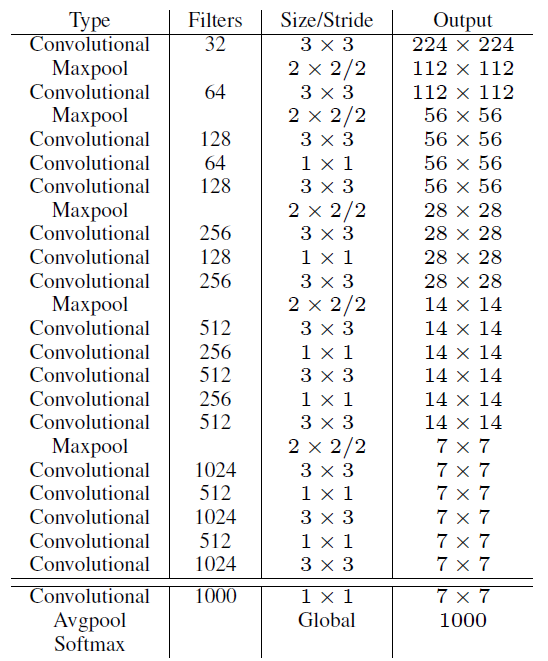
\includegraphics[width=.9\textwidth]{images/used_networks/yolov2_darknet.png}
\end{figure}
\chapter{Darknet-53}
\label{darknet-53}
\begin{figure}[H]
\caption{Darknet-53}
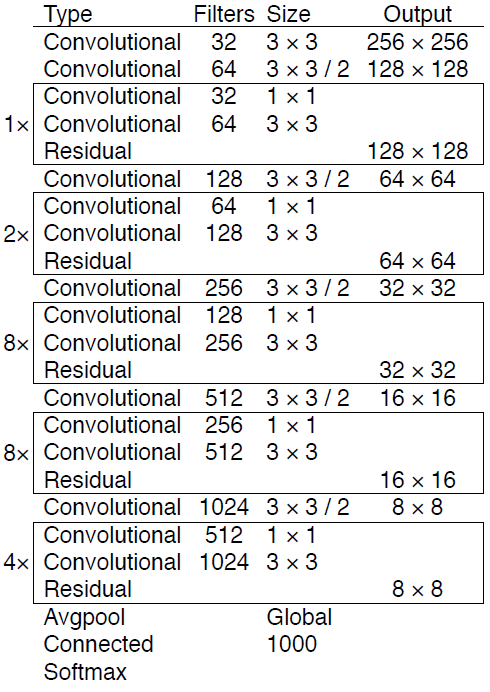
\includegraphics[width=.8\textwidth]{images/used_networks/yolov3_darknet.png}
\end{figure}

\chapter{Sample from videos used for evaluation}
\begin{figure}[H]
        \centering
        \subfloat[5.4 4K Camera Road in Thailand.mp4]{
                \centering
                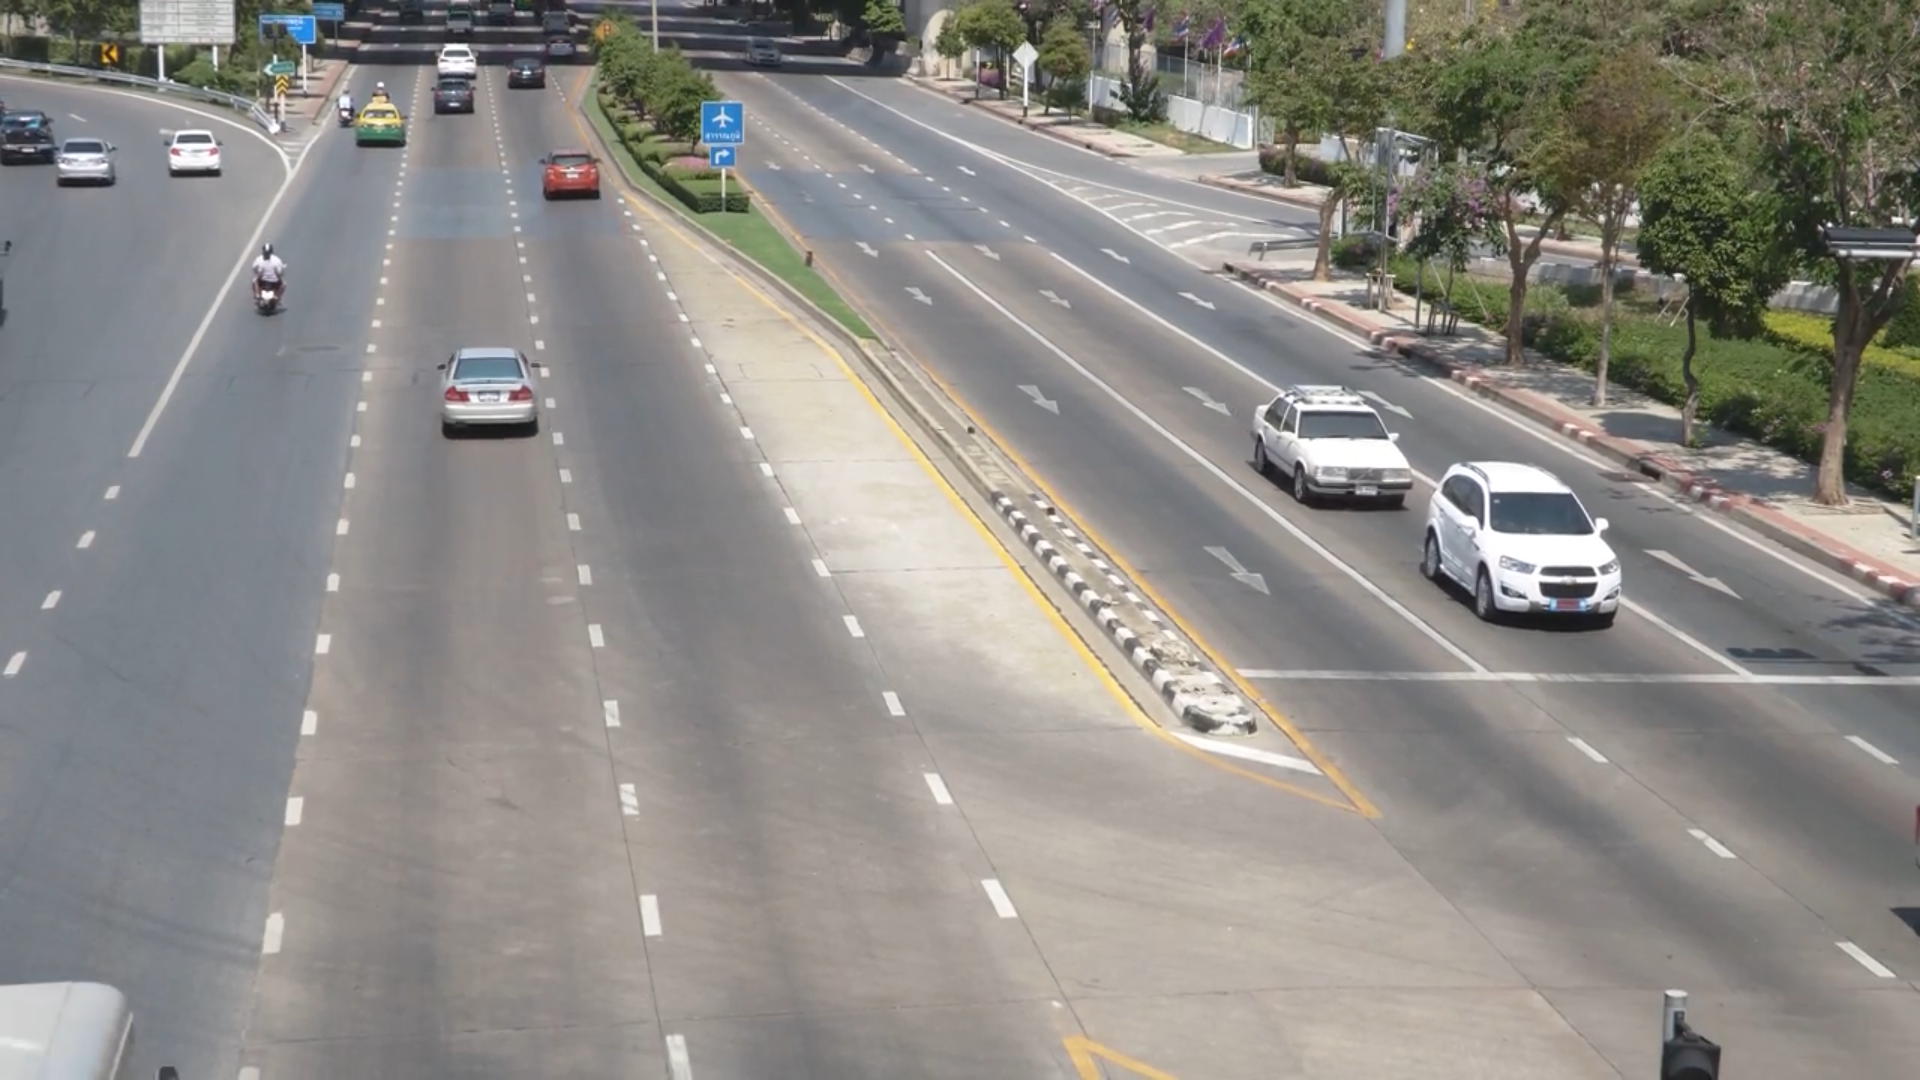
\includegraphics[width=.5\linewidth]{images/experiments/5_4.png}\label{fig:image1}
        }
        \subfloat[Cars Driving On Street.mp4]{
                \centering
                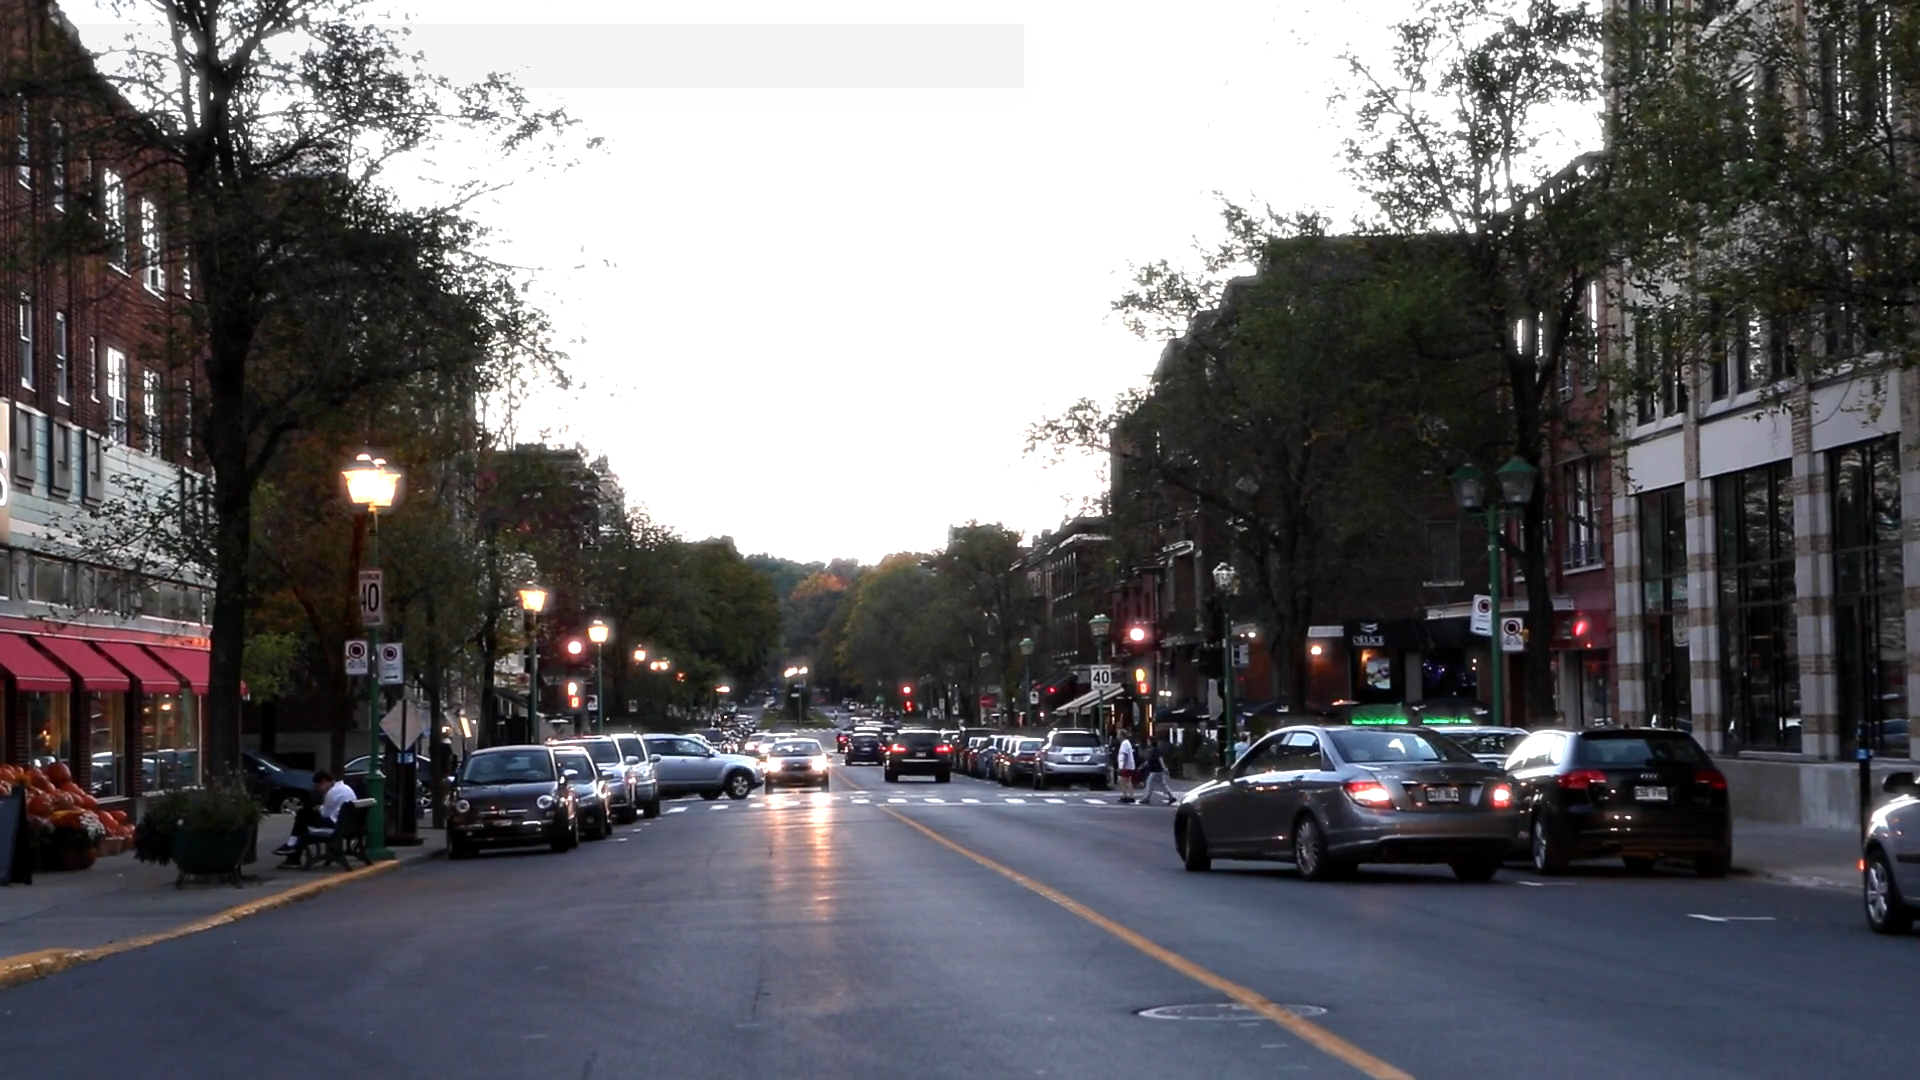
\includegraphics[width=.5\linewidth]{images/experiments/cars_on_streets.png}\label{fig:image1}
        }
        \hfill
                
        \bigskip
        \subfloat[Cars On Highway.mp4]{
                \centering
                
                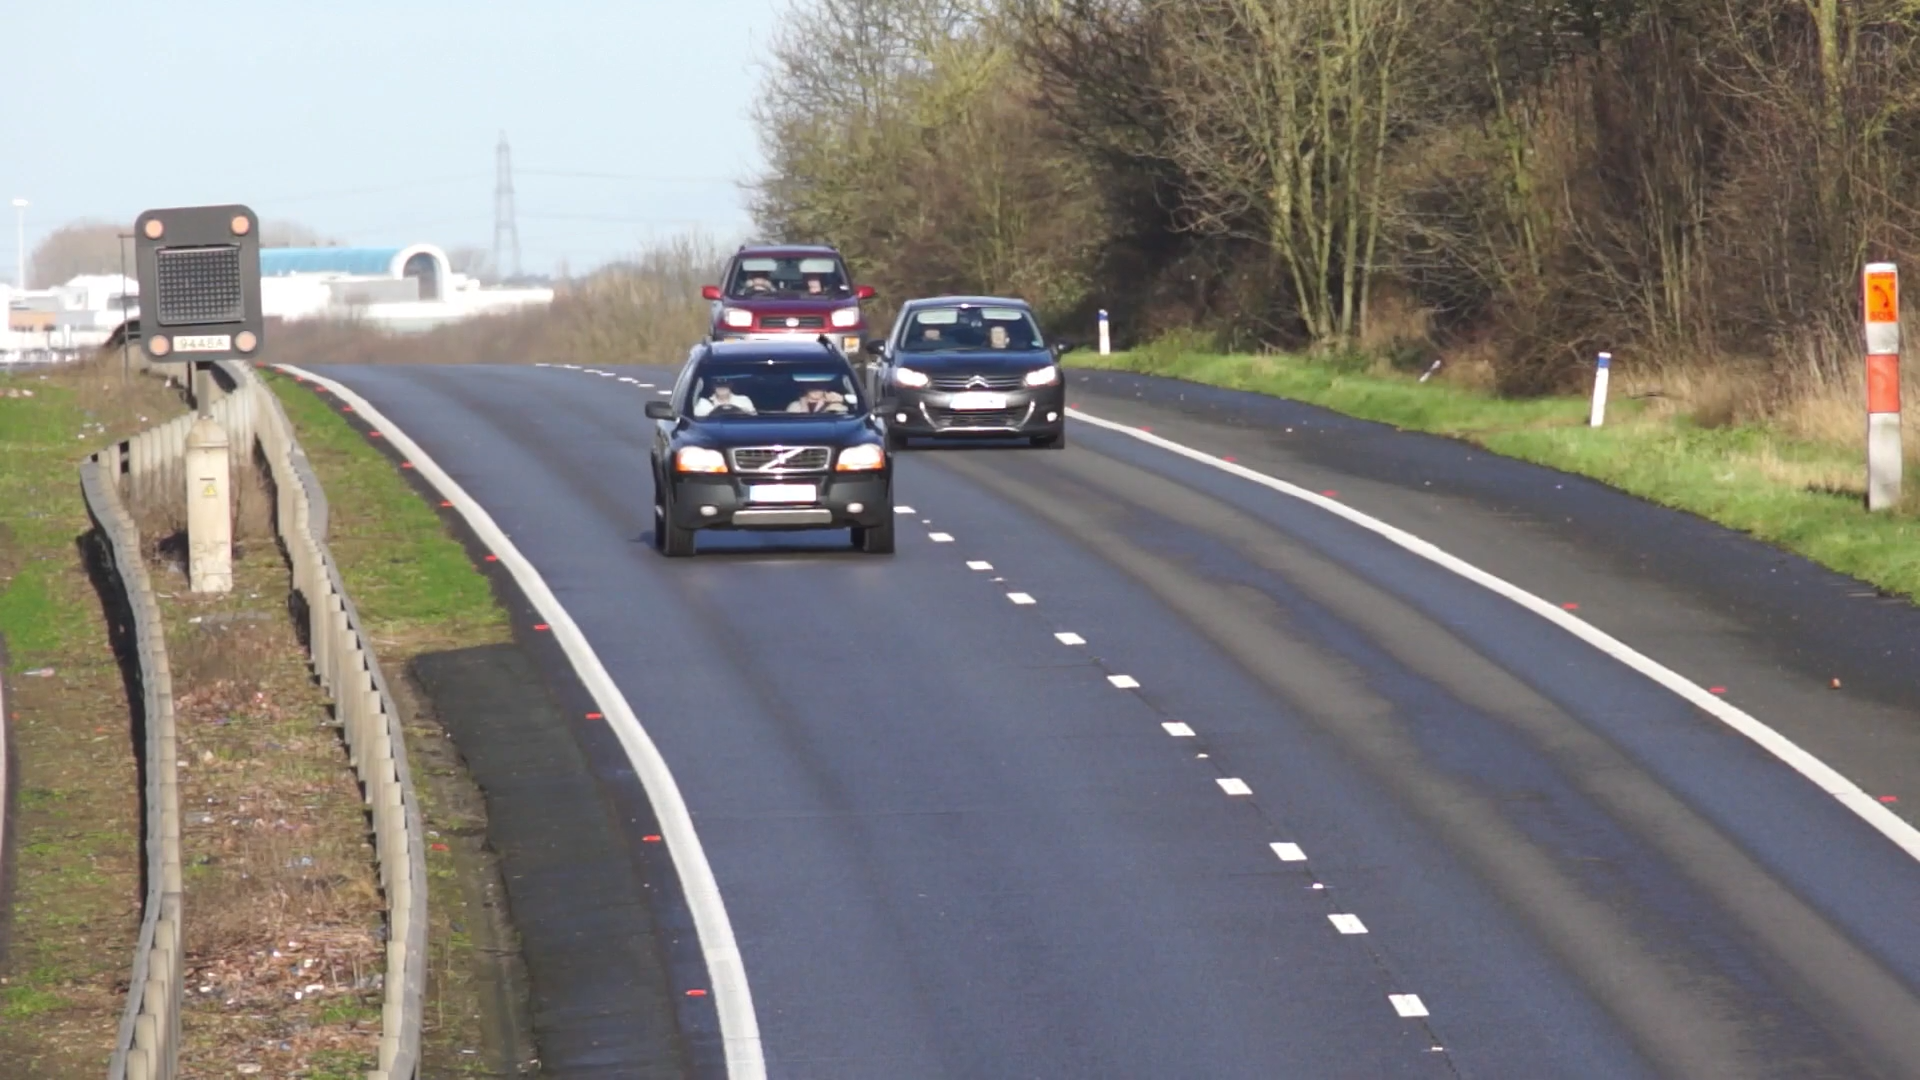
\includegraphics[width=.5\linewidth]{images/experiments/cars_highway.png}
                \label{fig:cars_highway}
        }
        \subfloat[Cars On The Road.mp4]{
                \centering
                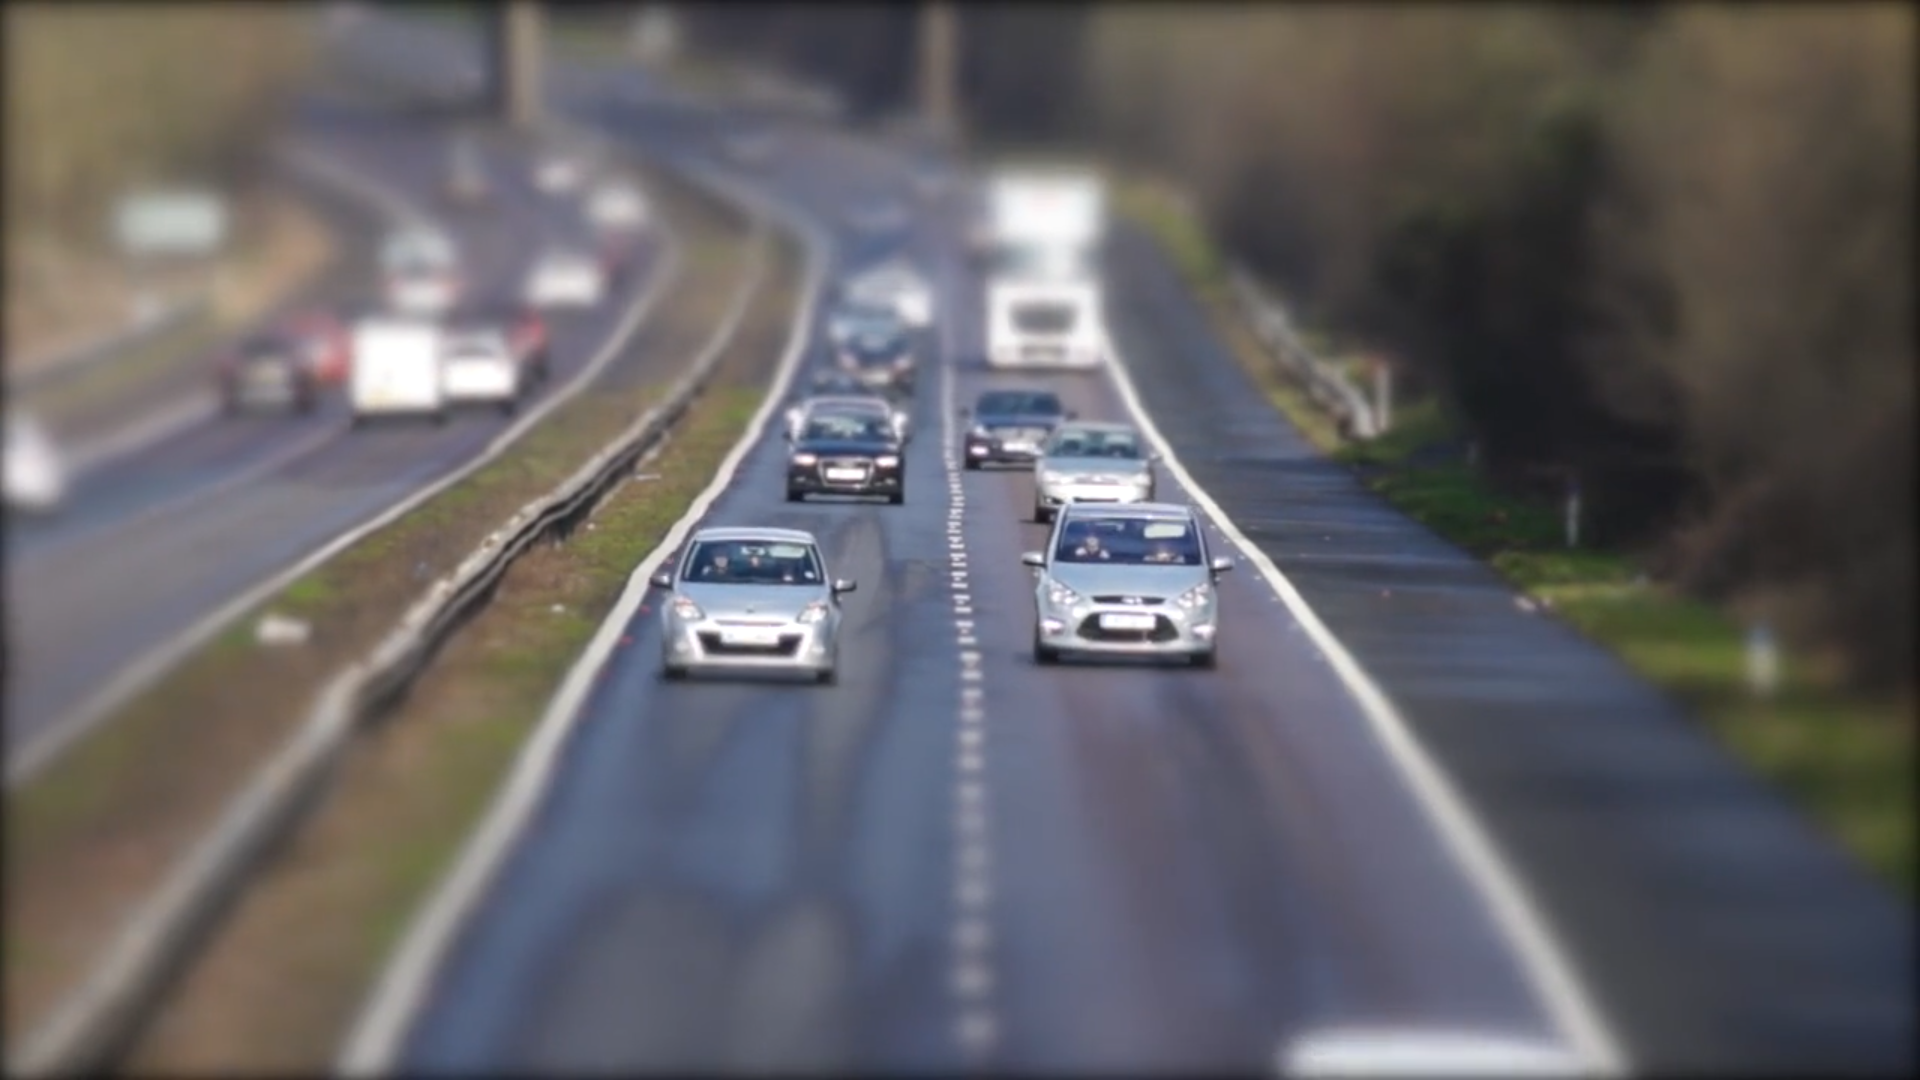
\includegraphics[width=.5\linewidth]{images/experiments/cars_road.png}\label{fig:image1}
        }
        \hfill
        \bigskip
        \subfloat[City Traffic.mp4]{
                \centering
                
                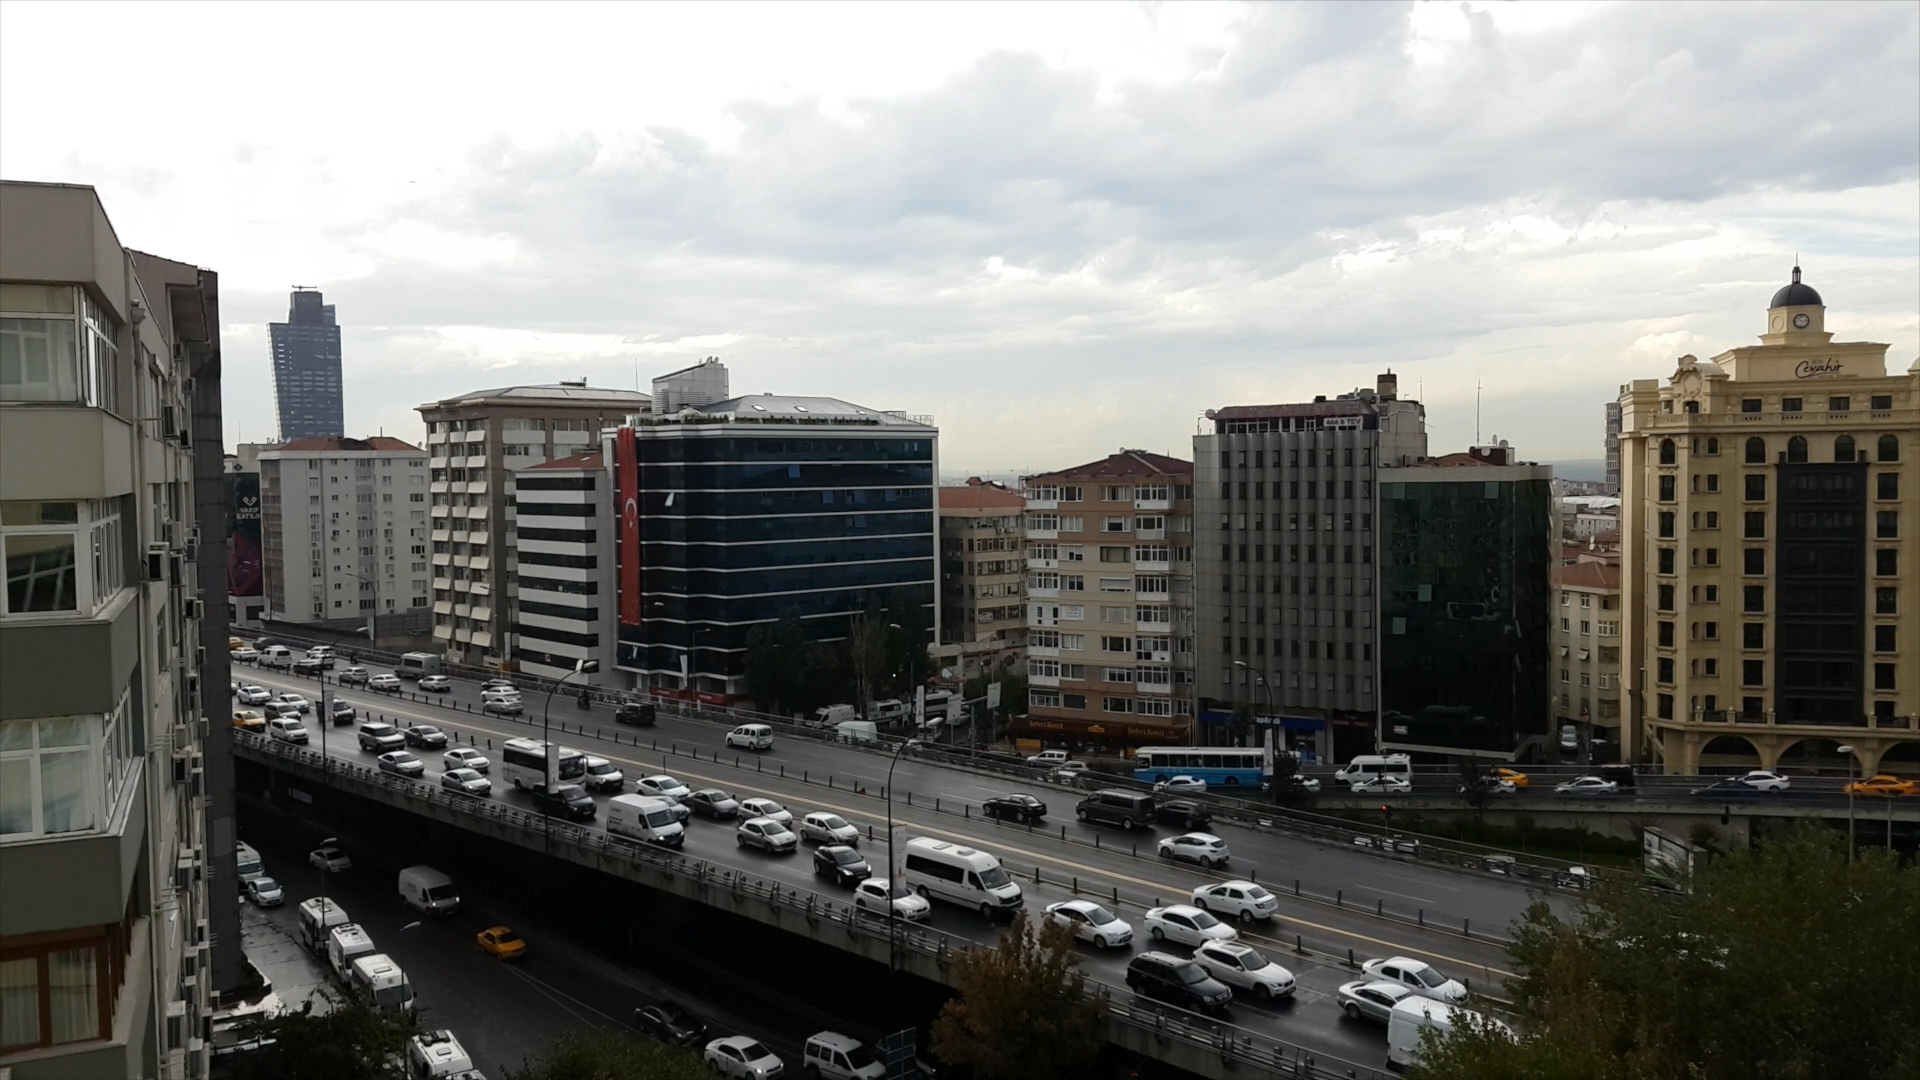
\includegraphics[width=.5\linewidth]{images/experiments/city_traffic.png}\label{fig:image1}
        }
        \subfloat[Day Traffic Sample Video Dataset.mp4]{
                \centering
                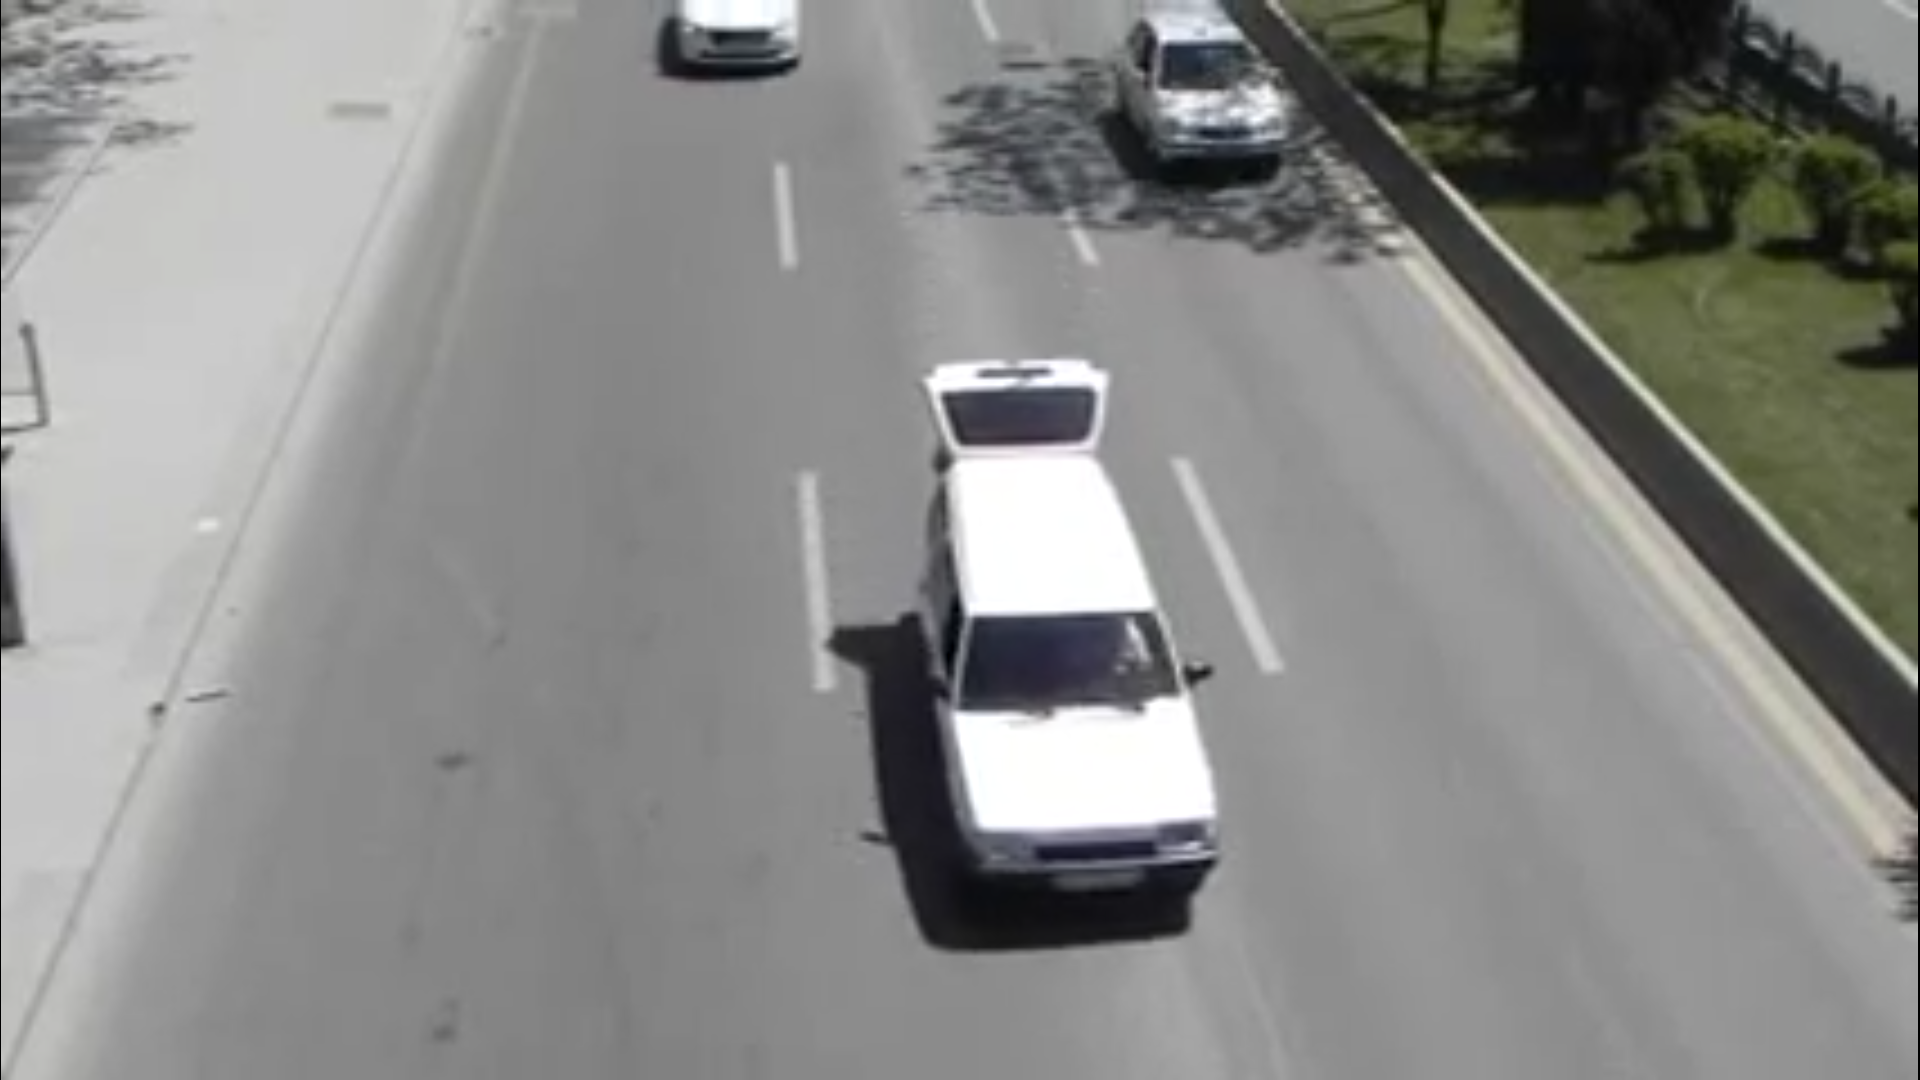
\includegraphics[width=.5\linewidth]{images/experiments/day_traffic.png}\label{fig:image1}
        }
        
        \end{figure}
        
        \begin{figure}
        
        \caption{Samples from used videos}
        \ContinuedFloat
        \subfloat[Pedestrian and Traffic, Human Activity Recognition Video ,DataSet By UET Peshawar.mp4]{
                \centering
                
                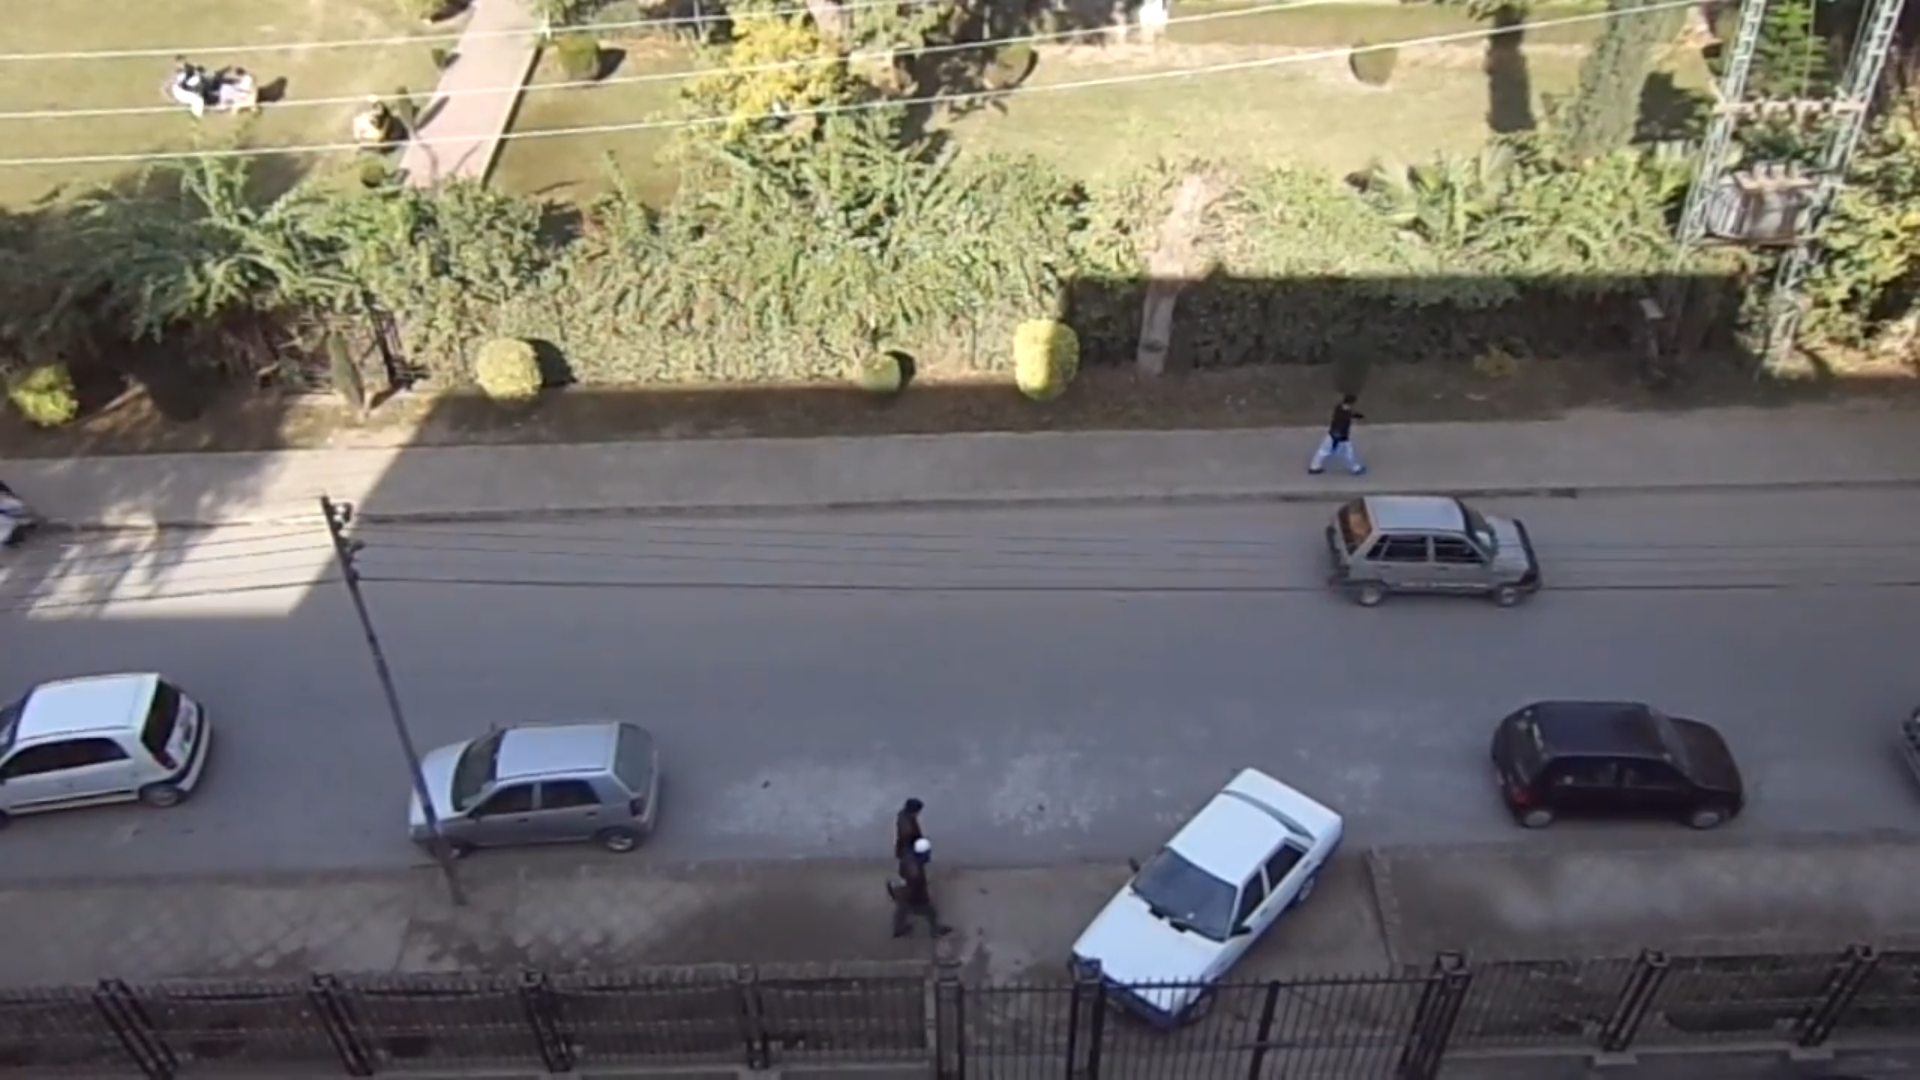
\includegraphics[width=.5\linewidth]{images/experiments/ped_humas_traffic.png}\label{fig:image1}
        }
        \subfloat[Pexels Videos 1601538.mp4]{
                \centering
                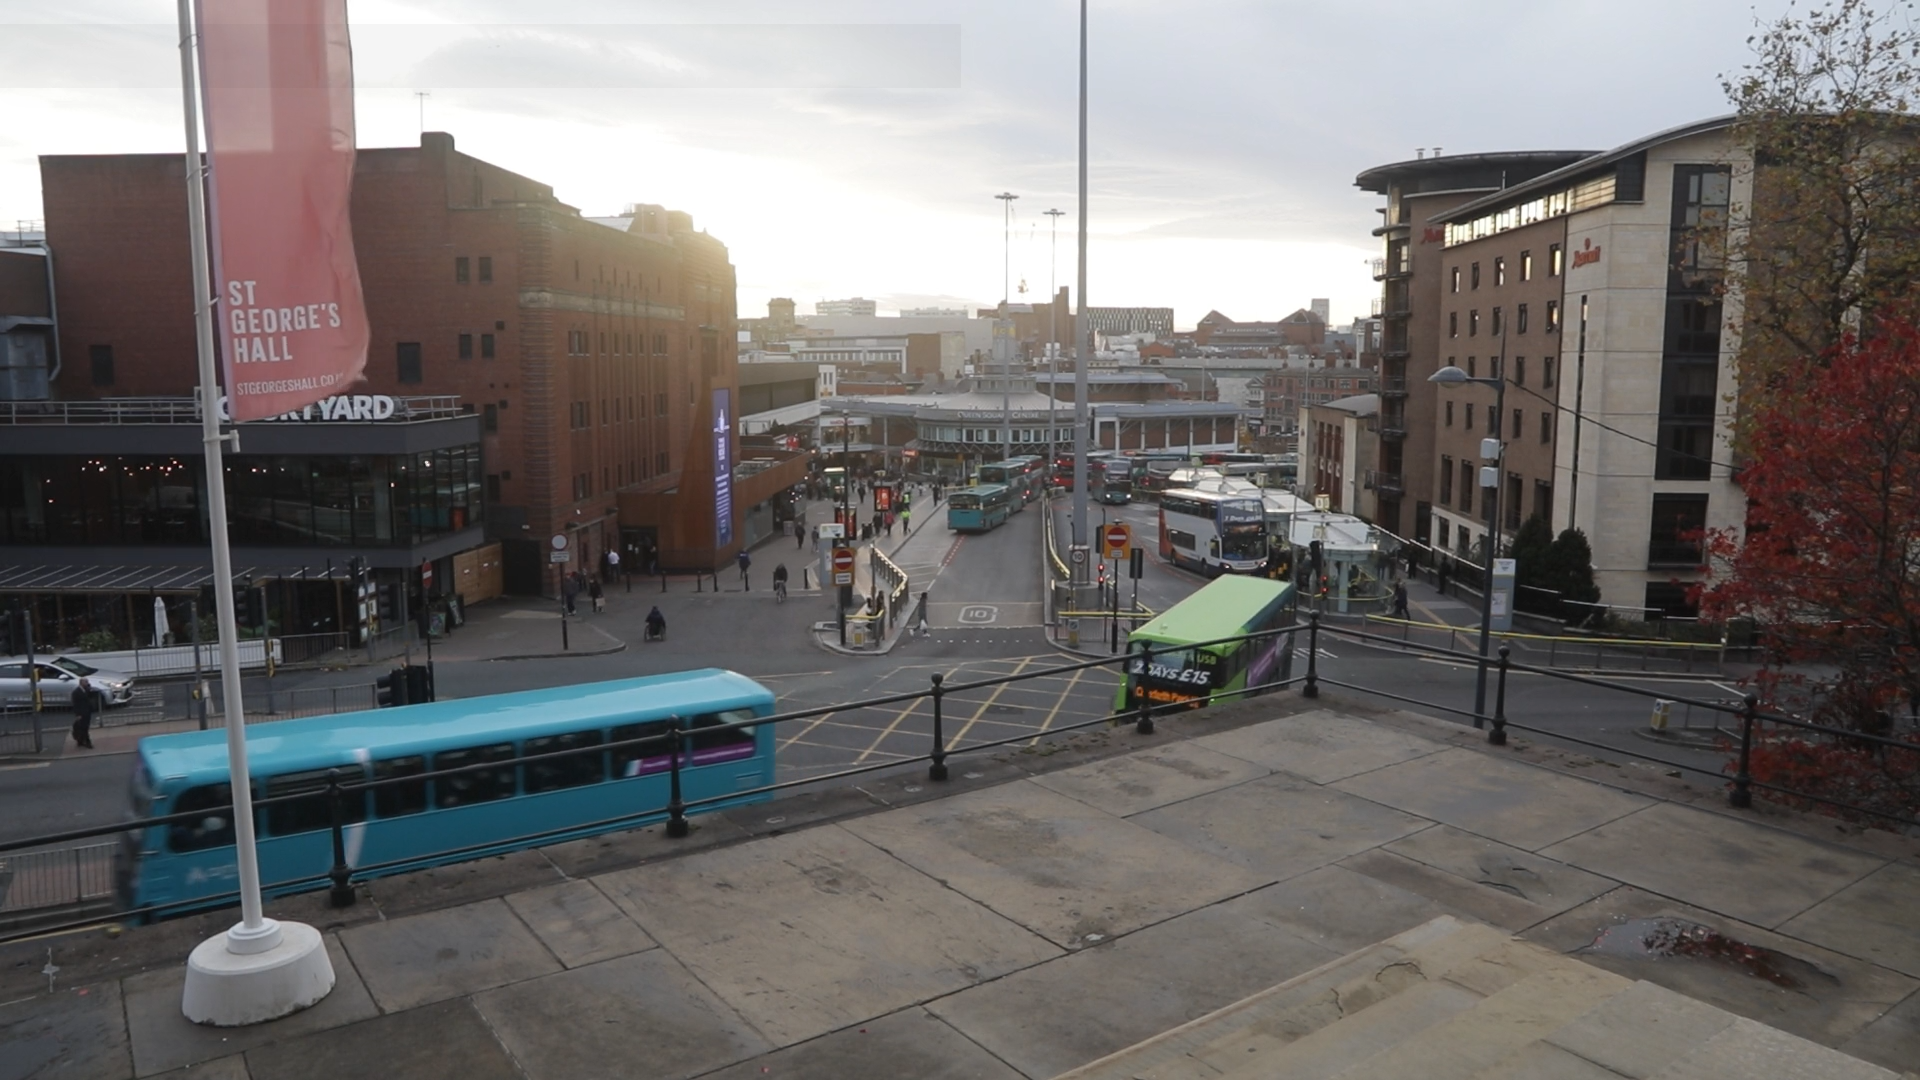
\includegraphics[width=.5\linewidth]{images/experiments/1601538.png}\label{fig:image1}
        }
        
        \hfill
        \bigskip
        \subfloat[Pexels Videos 2577.mp4]{
                \centering
                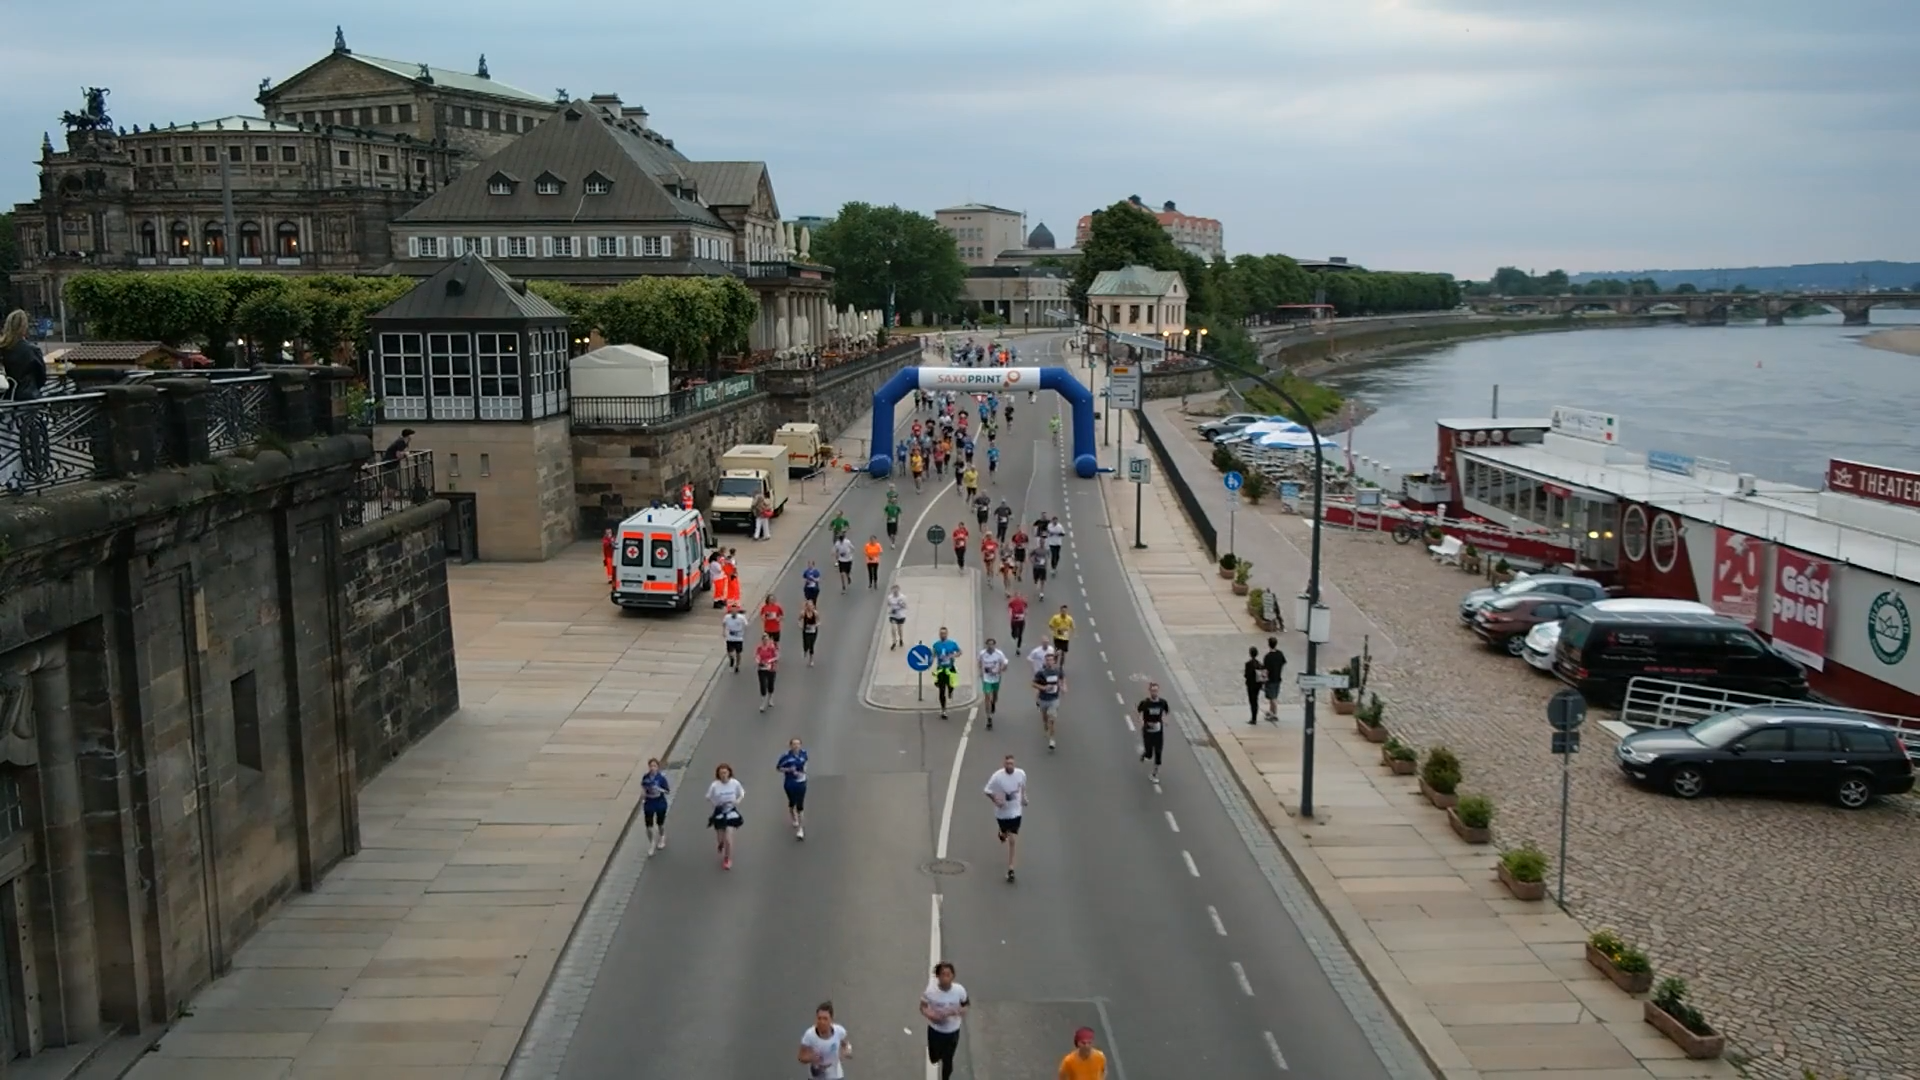
\includegraphics[width=.5\linewidth]{images/experiments/2577.png}\label{fig:image1}
        }
        \subfloat[Pexels Videos 2670.mp4]{
                \centering
                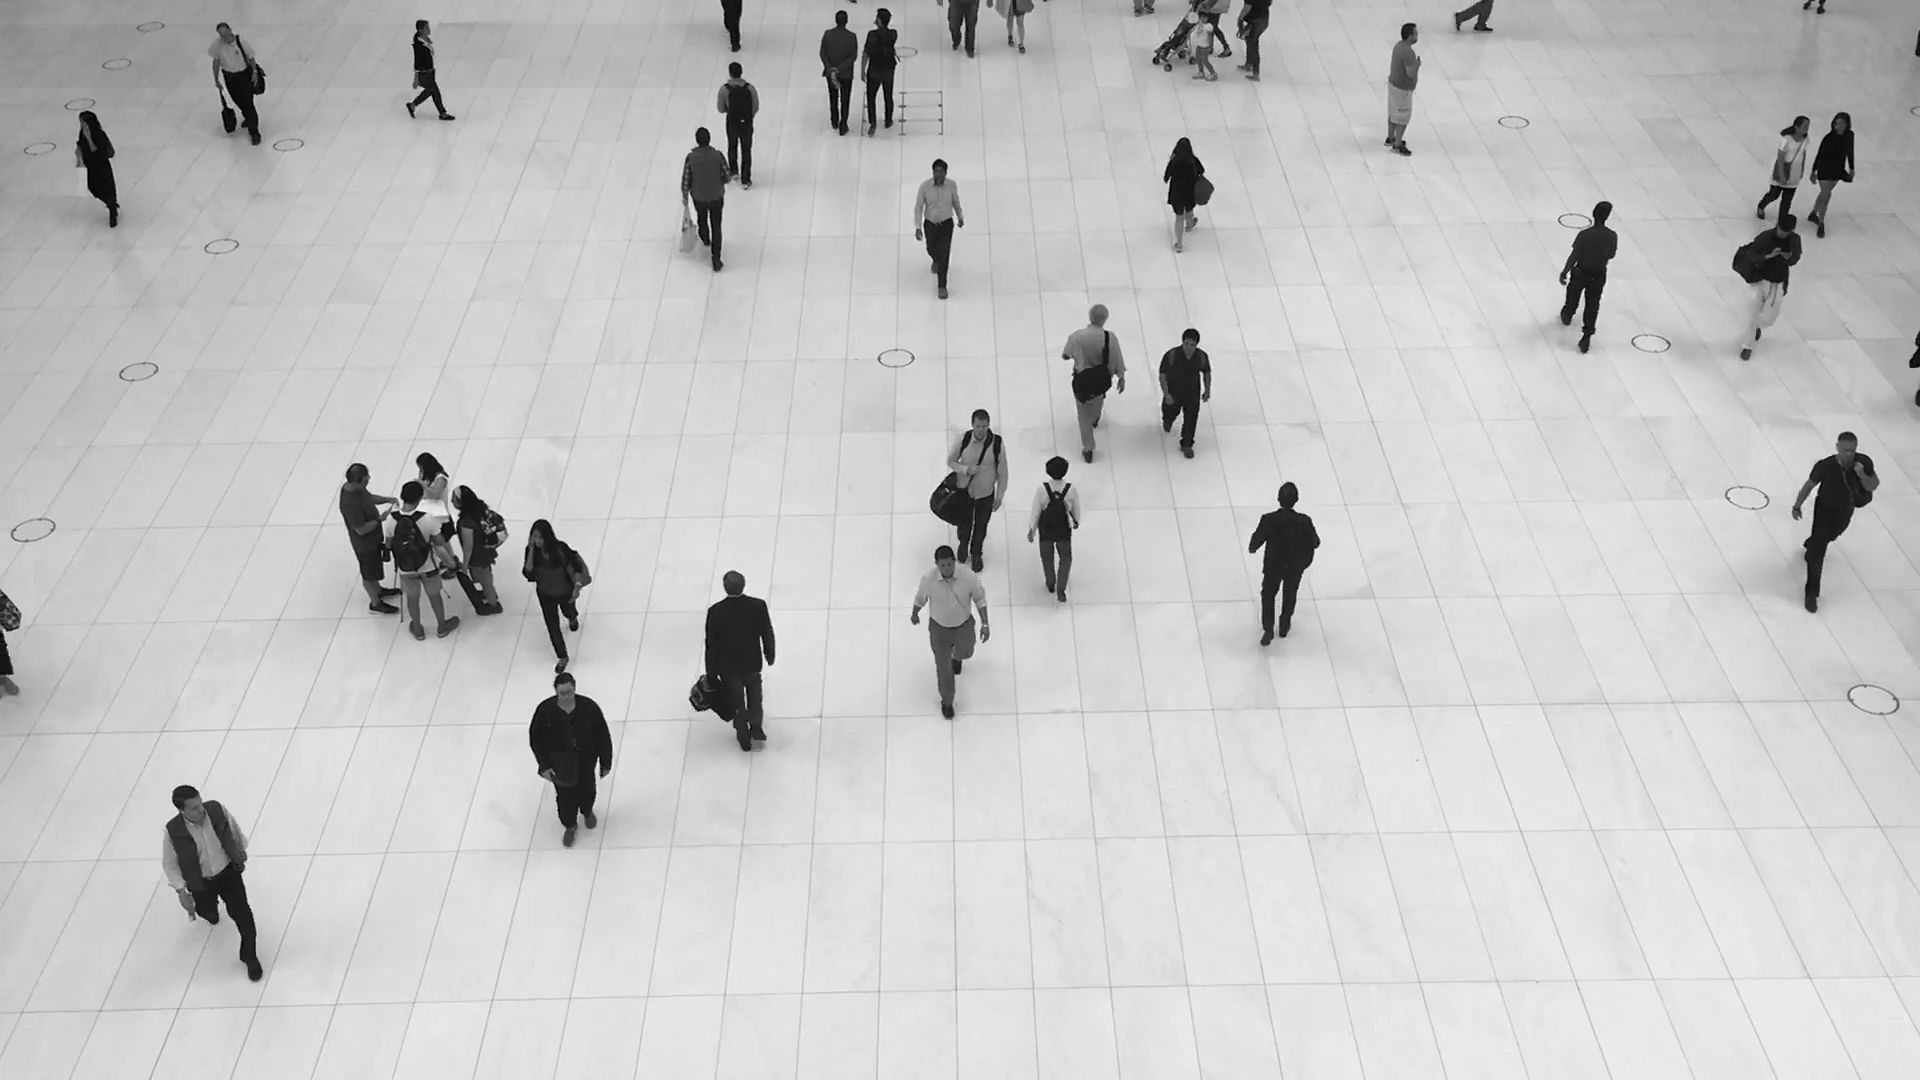
\includegraphics[width=.5\linewidth]{images/experiments/2670.png}\label{fig:image1}
        }
        \hfill
        \bigskip
        \subfloat[Pexels Videos 3047.mp4]{
                \centering
                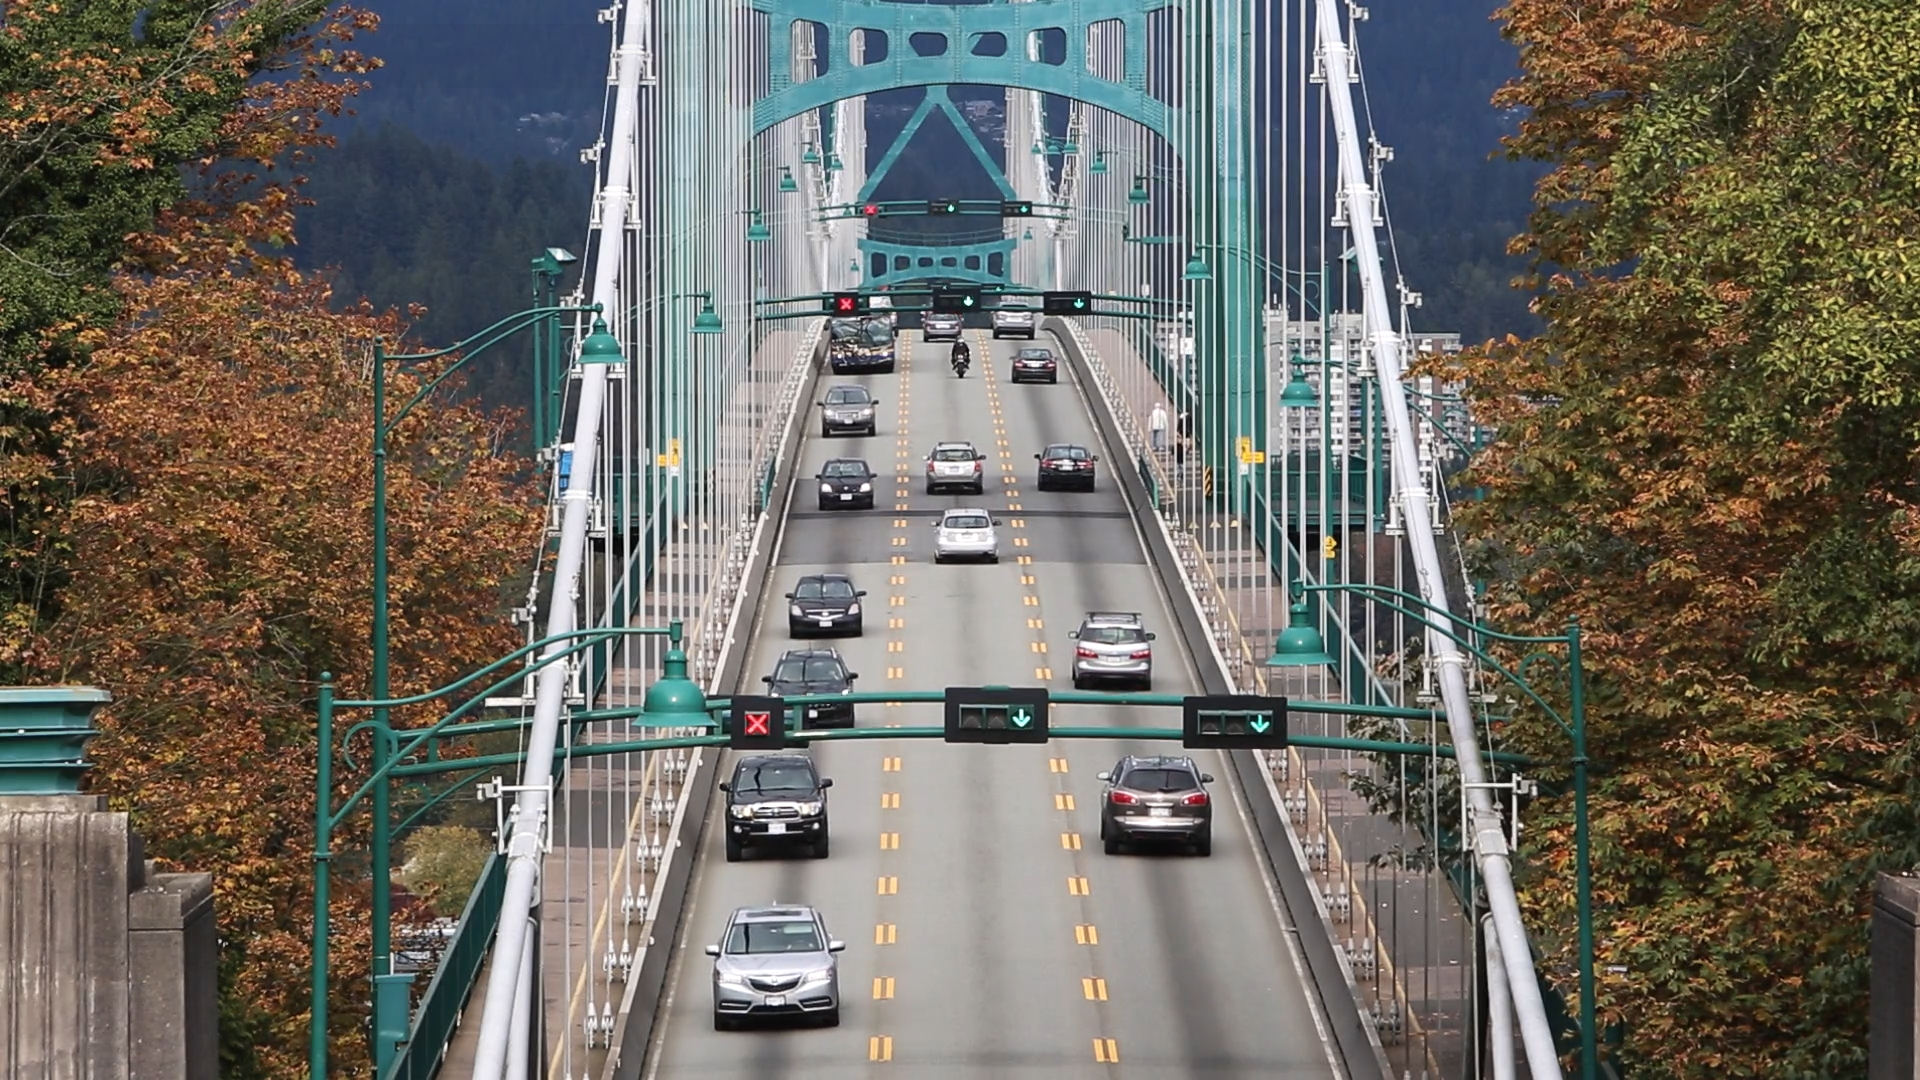
\includegraphics[width=.5\linewidth]{images/experiments/3047.png}\label{fig:image1}
        }
        \subfloat[Pexels Videos 948404.mp4]{
                \centering
                
                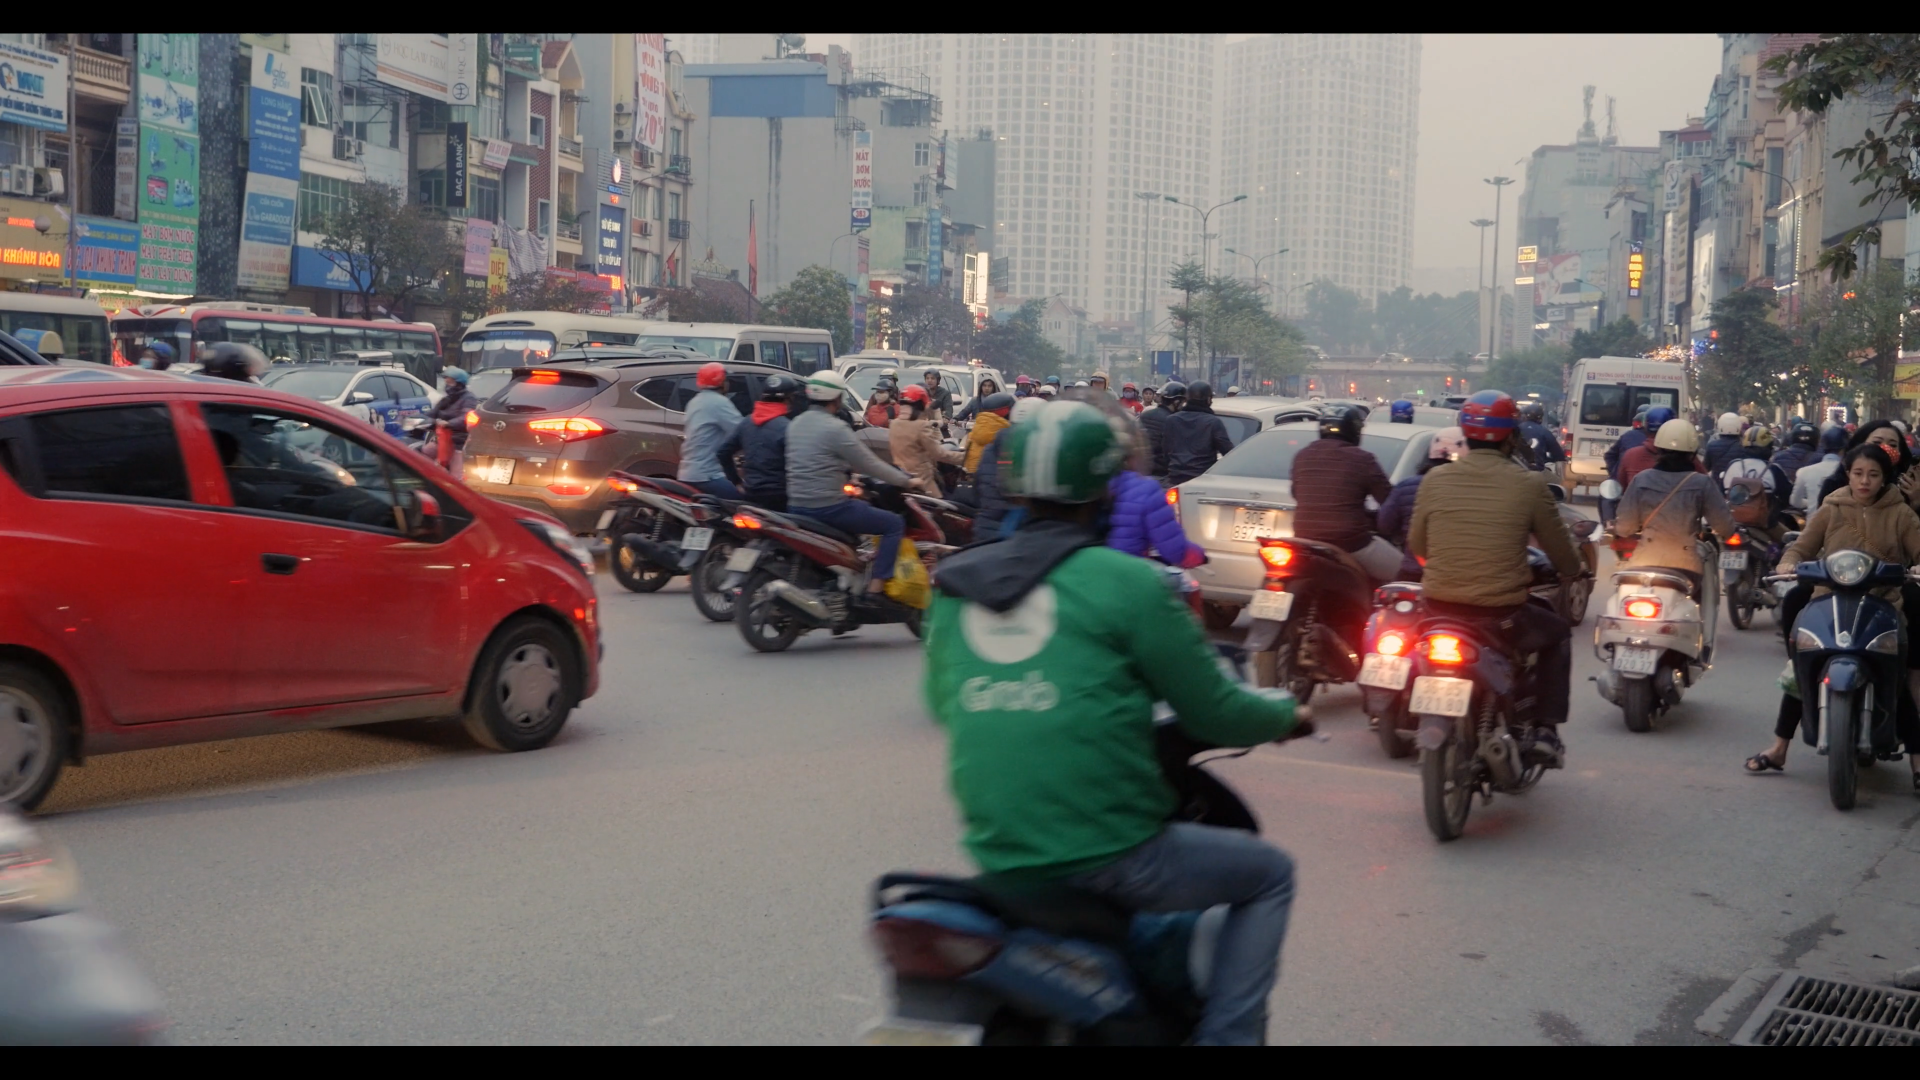
\includegraphics[width=.5\linewidth]{images/experiments/948404.png}\label{fig:image1}
        }
        \hfill
        \bigskip
        \subfloat[moderate\_traffic.mp4]{
                \centering
                
                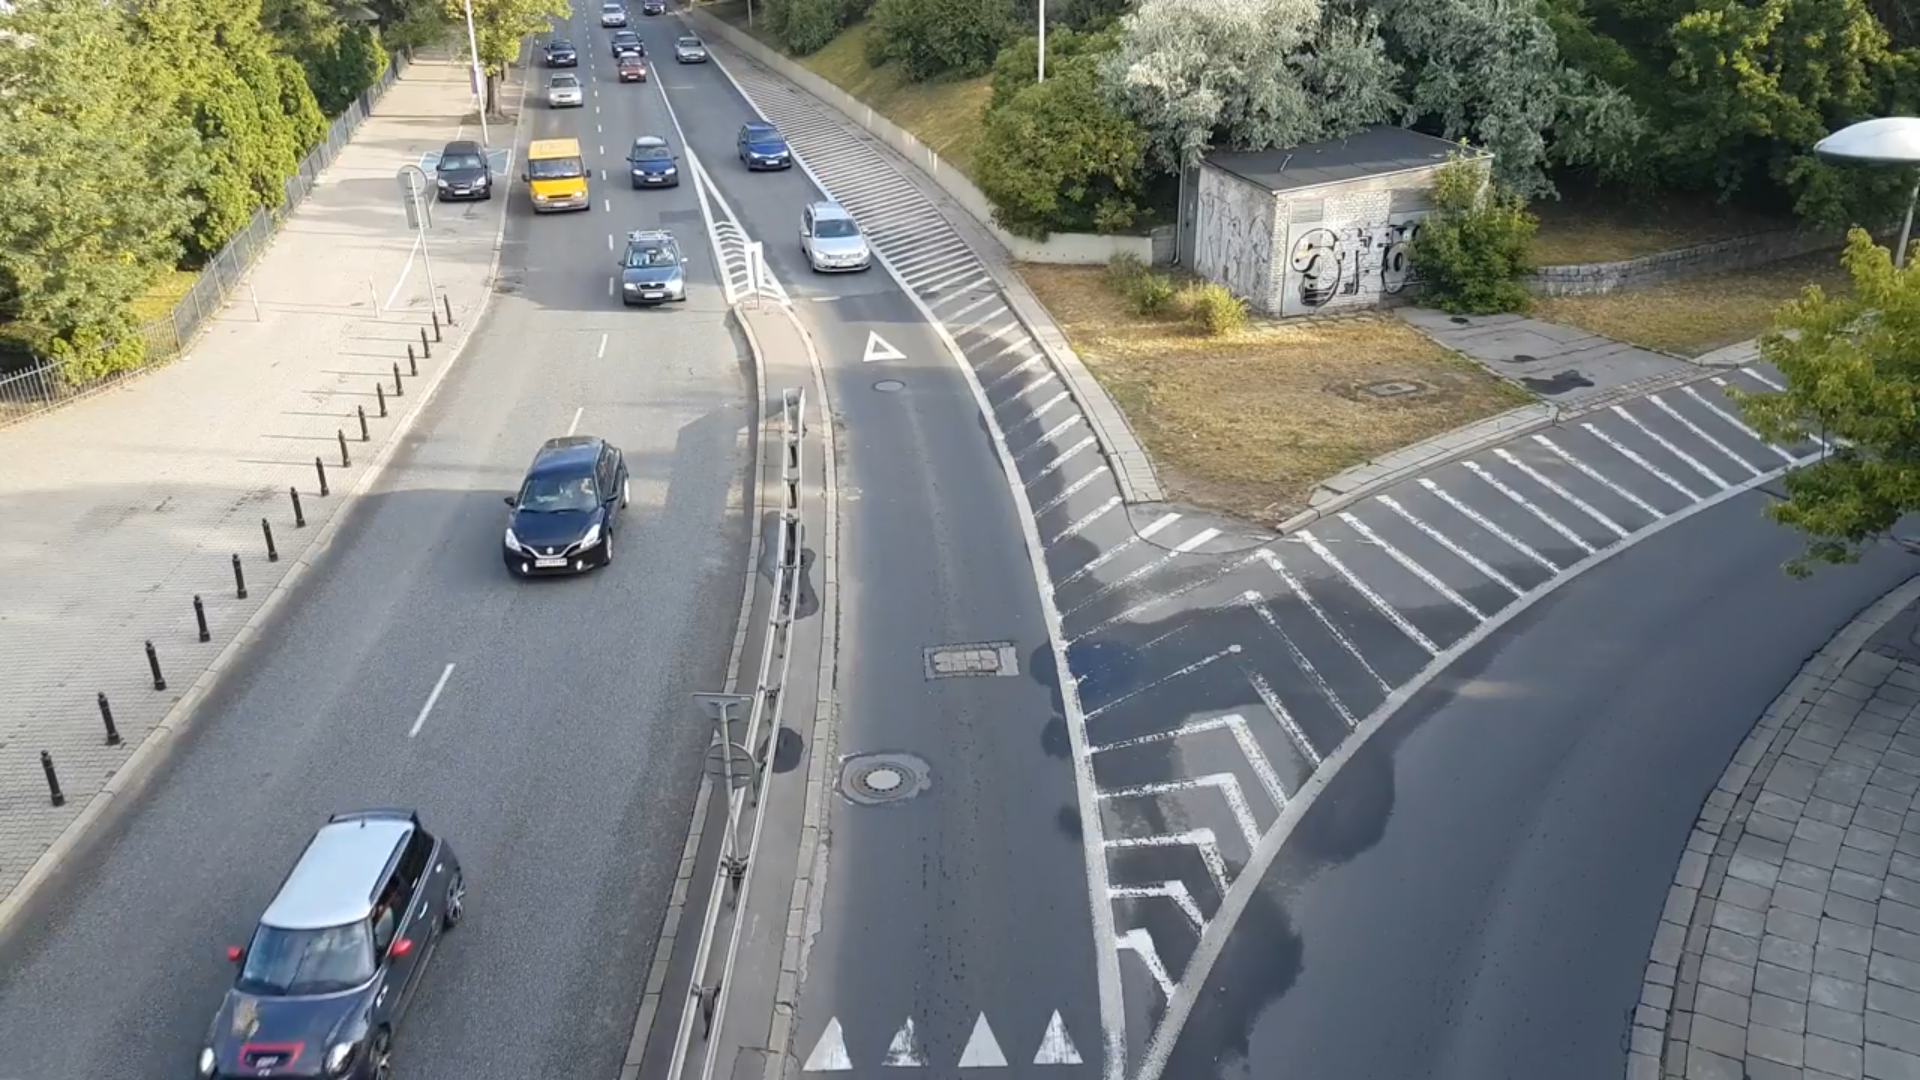
\includegraphics[width=.5\linewidth]{images/experiments/mod_traffic.png}\label{fig:image1}
        }
        \hfill
                \label{fig:samples}
\end{figure}
\iffalse
\chapter{Přehled algoritmů pro vyhýbání se překážkám}
\label{obstacle_avoidance}
\begin{figure}[H]
        \caption{Souhrn algoritmů pro vyhýbání se překážkám \cite[s. 287--290]{cite:20}}
        \label{korelace}
        \subfloat{\includegraphics[width=1\textwidth]{images/6/4.png}}
        \newline
\end{figure}
\begin{figure}[H]\ContinuedFloat
                \caption{Souhrn algoritmů pro vyhýbání se překážkám \cite[s. 287--290]{cite:20}}
        \subfloat{\includegraphics[width=1\textwidth]{images/6/1.png}}
        \newline
\end{figure}
\begin{figure}[H]\ContinuedFloat
                \caption{Souhrn algoritmů pro vyhýbání se překážkám \cite[s. 287--290]{cite:20}}
        \subfloat{\includegraphics[width=1\textwidth]{images/6/2.png}}
        \newline
\end{figure}
\begin{figure}[H]\ContinuedFloat        
        \caption{Souhrn algoritmů pro vyhýbání se překážkám \cite[s. 287--290]{cite:20}}
        \subfloat{\includegraphics[width=1\textwidth]{images/6/3.png}}
        \newline
\end{figure}
\fi
\printindex
\bibliographystyle{unsrt}
\bibliography{ctutest}
\end{document}
